

\chapter{Number}
\label{sec:NUM}

\section{Introduction}
\label{sec:NUM-intro}

According to \cite{Wies03} linguistic expressions denoting numerical concepts
come in three types: cardinal, ordinal and nominal. Cardinal numerals are those
usually  identified as modifiers: they are the cardinality of  sets of entities,
i.e. the numerical quantities.  Ordinal numerals are numerical ranks of entities
and nominal numerals are  numerical labels assign to entities.  A possible
number sequence
$N$ must satisfy the three following criteria: (i) All $x\in N$ must be
well-distinguished, (ii) $N$ must be a progression and (iii) (optional) $N$ must
be
infinite \citep[304]{Wies03}.  

This chapter investigates  linguistics aspects of Chakali numerical concepts.
First the cardinal numeral system is described. In section
\ref{sec:NUM-enum}  the enumerative forms are introduced. Next,  how
distribution and repetition are expressed when they involve numerical concepts
is considered.
Section
\ref{sec:NUM-partitive} looks at both the ordinal and nominal numerical
concepts.  The relation between number and currency is  discussed in section
\ref{sec:NUM-currency}.  In section \ref{sec:NUM-gramarith}, a 
formalization  proposes composition rules which are responsible for
generating  complex numerals. The last section  is a digression into
comparative  linguistics  where a partial Southwestern Grusi (SWG)
clustering is proposed.

%and then interpreted as reflecting recent stages in the evolution of Proto-SWG.

%In comparing with other GSW languages, we argue that the Chakali numerical
%system is an innovation of an original *GSW  base-5 system. 

\section{Atomic and Complex Numerals}
\label{sec:NUM-bas-comp}

To keep the technical terms as simple and relevant as possible, I use the
terminology  found in \cite{Gree78b}. The same source influenced our
discovery
procedure: ``To each numeral is assigned one or more numbers based on morphemic
identifications, and the arithmetical functions are inferred''
\cite[263]{Gree78b}. The simplest lexicalisation of a number is called a numeral
atom, whereas a complex numeral is an expression in which  one can infer at
least one arithmetical function.  A numeral atom can stand alone or can
be combined
with another numeral, either atomic or complex, to form a complex numeral. Atoms
are treated as  those forms which are not decomposable morpho-syntactically at a
synchronic level. Table \ref{tab:numeralatoms} displays the twelve
atoms of the numeral system.

 \begin{table}[!h]
  \caption{Atomic numerals from 1 to 8, 10, 20, 100 and 1000
\label{tab:numeralatoms}}
   \centering
{\I
  \begin{tabular}{ll}
\Hline
Chakali &     English \\ \hline
 dɪ́gɪ́máŋá & one \\
álɪ̀ɛ̀ &two   \\         
átòrò &three   \\         
ànáásɛ̀ &four  \\         
 àɲɔ̃́ &five  \\         
  álòrò   &six  \\         
  àlʊ́pɛ̀   &seven \\         
  ŋmɛ́ŋtɛ́l &eight  \\        
% dɪ́ɡɪ́tʊ̀ʊ̀ &nine   \\         
  fí &ten \\ 
 màtʃéó  &twenty   \\         
  kɔ̀wá (pl.  kɔ̀sá)   & hundred(s)  \\
  tʊ́sʊ̀  (pl.  tʊ́sà) &thousand(s)    \\         
\Hline
\end{tabular}
}
%\vspace{1.1cm}

 
\end{table}

The term for `one'  is expressed  as  {\S dɪ́gɪ́máŋá},  but  {\S dɪ́gɪ́ɪ́}
alone  can also
be used. In general, the meaning associated with the morpheme {\S máŋá} is
`only', e.g.  {\S bahɪɛ̃ maŋa n̩ na} {\it old man-only-I-saw} `I saw only an old
man'. 
 The number 8 is designated with  {\S ŋmɛ́ŋtɛ́l}, an expression which is also
used to refer to the generic term for  `spider'.  Whether they are homonyms,
or whether
 their
meanings enter into a polysemous/heterosemous relationship is unclear. Another
characteristic is that the higher
numerals 100 and 1000  have their own plural form. From the
atoms,  the complex numerals are now examined.
 
The arithmetical functions inferred are called operations. In Chakali three
types of operation are found: addition, multiplication and subtraction. An
operation always has two arguments which are identified in
\cite{Gree78b} as: 

\vspace{3ex}

\begin{tabular}{ll}
{\bf Augend:} & A value to which some other value is
added.\\
{\bf Addend:} & A value which is added to some other
value.\\
{\bf Multiplicand:} & A value to which some other
value multiplies.\\

{\bf Multiplier:} & A value which is multiplied to
some other value. \\

{\bf Subtrahend:}  & The number subtracted.\\
{\bf Minuend:}  & The number from which subtraction takes
place.\\
\end{tabular}
\vspace*{10pt}


The numeral {\S dɪ́ɡɪ́tʊ̀ʊ̀} expresses the number 9. It is the only
expression associated with subtraction.  The subtrahend is the expression {\S
dɪɡɪɪ} `one'.   In {\S dɪ́ɡɪ́tʊ̀ʊ̀},  the last syllable   is analyzed
as the
operation. It may originate from the state predicate  {\S tùwó} which is
translated 
`not exist'  or `absent from' (section \ref{sec:GRM-loc-cl}). Thus, assuming the
covert minuend 10, the numeral
expression receives the functional notation [1 {\sc absent from} 10], or 10
minus 1.  The number 9 may also be expressed as {\S sàndòsó}  (or
{\S sandʊsə} in Tuosa and Katua). This expression is
used by some individuals in Ducie, Tuosa and Katua, all of them from the most
senior generation.  One language consultant
associates  {\S sàndòsó} with the language of women, but his claim is not
sustained by other language consultants. For the number 9, \citet[33]{Good54}
reports
{\S saanese}
from the village Katua and  \citet[117]{Ratt32b} puts {\S sandoso} as the form
 for 9 in Tampulma. 

 
A proper  treatment of  atomic versus  complex numerals   relies  on evidence as
to whether
a numeral is synchronically  decomposable. In  that spirit,  numbers from 
11 to 19 are expressed with  complex numerals:  one piece of evidence, which is
presented in section \ref{sec:GRM-gender} and repeated in section
\ref{sec:NUM-npstruc}, comes from the gender agreement between the head of a
noun phrase and the
cardinal numeral functioning as modifier.  Table \ref{tab:numral11-19}
provides the  numerals from 11 to 19 with a common structure
[fi_{10}-d(ɪ)-X_{1-9}]. 




  \begin{table}[!h]
  \caption{Complex numerals from 11 to 19  \label{tab:numral11-19}}
   \centering
{\I
  \begin{tabular}{ll}
\Hline
 Chakali & English   \\ \hline
 fí dɪ dɪ́ɡɪ́ɪ́ & eleven  \\
 fí dɪ álìɛ̀ & twelve  \\
  fí dɪ átòrò &  thirteen \\
fí dɪ ànáásɛ̀ &  fourteen \\
 fí dɪ àɲɔ̃́ &  fifteen \\
 fí dɪ álòrò  & sixteen  \\
fí dɪ àlʊ̀pɛ̀ &  seventeen \\
  fí dɪ ŋmɛ́ŋtɛ́l  &  eighteen \\
  fí dɪ dɪ́ɡɪ́tʊ̀ʊ̀ &  nineteen \\

\Hline
\end{tabular}
}


\end{table}

The criterion employed for  the distinction between augend and addend is that an
augend is serialized, that is, it is the expression which is constant in a
sub-progression. This expression is called the base. In the progression from 
eleven to nineteen shown  in  table  \ref{tab:numral11-19},  the augend is {\S
fi} and the addends are the expressions for one to nine. Given the
above definition of a base,  the expression 
{\S fi} is  the base in complex
numerals  from 11 to 19. The operator for
addition is {\S dɪ} and its vowel surfaces only when the
 following word starts with a consonant (i.e. {\S fídɪ̀ŋmɛ́ŋtɛ́l} `18', but
{\S
fídànáásɛ̀} `14').




Table \ref{tab:numeral21-99} provides the sequences of  numeral atoms
forming the complex numerals referring to  numbers from 21 to 
99. 



  \begin{table}[!h]
  \caption{Complex numerals from 21 to 99  \label{tab:numeral21-99}}
  \centering
{\I
  \begin{tabular}{lll}
\Hline
Number  & Numeral & Meaning  \\ \hline
    
21-29& atom {\S anɪ} atom &  20  + (1 through 9) \\ 
30  &  atom  {\S anɪ} atom  & 20  + 10\\   
31-39&  atom {\S anɪ} complex  & 20  + (11 through 19)     \\      
40 &  atom  atom & 20 $\times$    2 \\
41-49&   atom  atom  {\S anɪ} atom &  20 $\times$  2  + (1 through 9) \\     
50 &  atom  atom  {\S anɪ} atom & 20 $\times$ 2 + 10 \\ 
51-59 & atom  atom  {\S anɪ} complex &20 $\times$ 2  + (11 through 19)\\ 
60 & atom  atom & 20 $\times$ 3\\ 
61-69 & atom  atom {\S anɪ} atom  &20 $\times$ 3 + (1 through 9) \\
70 &  atom  atom  {\S anɪ} atom& 20 $\times$ 3 + 10\\ 
71-79 &atom  atom  {\S anɪ} complex  &20 $\times$ 3   + (11 through 19)\\ 
80 & atom  atom  & 20 $\times$ 4\\ 
81-89 & atom  atom {\S anɪ} atom&20 $\times$ 4 + (1 through 9)\\ 
90 &  atom  atom  {\S anɪ} atom&20 $\times$ 4 + 10 \\ 
91-99 & atom  atom  {\S anɪ} complex& 20 $\times$ 4   + (11 through 19)\\      
\Hline
\end{tabular}
}


\end{table}


% Mathematics The number by which another number is multiplied. In 8 X 32, the
%multiplier is 8.

Table \ref{tab:numeral21-99} shows us that either (i) an atom can follow another
atom without any intervening particle  or (ii) the particle {\S anɪ} can step in
between two atoms, or one atom and one complex numeral. Case (i) is understood
as a phrase which multiplies the numerical values of  two atoms. For
instance, 
{\S matʃeo atoro} [20
3] results in the product `sixty', and not the sum `twenty-three',   as in
English. All numeral phrases from 20 to 99 use {\S matʃeo} in their formation. 
In case (ii),  the particle {\S anɪ} is treated as an operator similar to the
semantics of  `and' in English numerals since it adds the value of each
argument, either atom or complex.  The same form is also found in noun phrases
expressing the union of two or more entities (see section
\ref{sec:GRM-conjunc-nom}).
The vowels of {\S anɪ} are reduced when preceded and followed by
vowels.

The same criterion applies for the distinction between multiplier and
multiplicand: the latter  is identified on the basis of what Greenberg calls
`serialization'. So, a  base may be   a serialized multiplicand as well since it
is the constant term in the complex expressions involved in a sub-progression.
The expression  {\S matʃeo} is therefore the base in complex numerals  from 21
to 99. The composition of complex numerals is summarized in table
\ref{tab:threecompo} and  a formal rendering is given in section
\ref{sec:NUM-gramarith}.


\begin{table}[h]
\caption{General structure of complex numerals  \label{tab:threecompo}}
  \centering

\begin{tabular}{lll}
\Hline
  Argument & Meaning & Restriction\\
\hline
 ($y$)   $x$   tuo  & subtraction  &$y={10}$\\
&& $x={1}$\\ 
   $x$ anɪ $y$ & addition  &$x>y$ \\
$x$ dɪ $y$  & addition &$x={10}$ \\
&& $y={1 \textrm{-}9}$\\ %left sister x is 10

$x y$ & multiplication &$x=20$  \\
&& $y={2,3,4}$\\ %right sister y smaller than left sister x
$x y$  & multiplication  &$x={100}$ \\
&& $y={2 \textrm{-}9}$\\ %left sister x is 10
$x y$  & multiplication  &$x={1000}$ \\
&& $y={2 \textrm{-}999, 1000}$\\ %left sister x is 10
\Hline
\end{tabular}
\end{table}


As earlier mentioned, in subtraction  the minuend $y$ is covert. The only case
of subtraction 
is the numeral {\S dɪ́ɡɪ́tʊ̀ʊ̀} `nine'.  Both
addition  and multiplication take two overt arguments  $x$ and
$y$. They
are presented in the first column  of table \ref{tab:threecompo} with their
surface linear order. The operator for addition {\S dɪ} is used only  for the
sum of 10 and numbers between 1 and 9. The form {\S anɪ} is found in a variety
of structures, but it restricts the right sister $y$ to be lower than the left
sister $x$. In multiplication  the value of the argument $y$ 
depends on the
value of $x$. For the numerals designating  2000 and above, the argument $x$
must be
the atom {\S tʊsʊ} `thousand' and $y$  any atom or complex numeral between 2 and
999. There are no terms to express  `million' in Chakali. One can hear 
individuals at the
market  using the English word `million' when referring to  currency. According
to my consultants,  the expression {\S  tʊsʊ tʊsʊ} [1000 $\cdot$ 1000]
`million' was
common, but became archaic even before the change of currency  in July 2007
(see comments in section \ref{sec:NUM-gramarith}).
Examples of numerals are presented in (\ref{ex:diffstrings}).
%The possibly foreign origin of {\F tʊsʊ} '1000' is not yet established.

%\pagebreak

%The latter rule is  involved in the composition of the complex numeral given in
% (\ref{ex:21231}), that is $[\ipaT{tUsI}  [matʃeo  \  \ipaT{anI} \ 
%dɪgɪmaŋa]_{A}]_{B_c}$ `21 000'.

%\pagebreak

%I treat Chakali 11-19 as composition, but one could also treat those nine
%numerals as atoms. That is because the only structures in which \ipaT{di} is
%found are in the composition of  11 to 19 (e.g. fi\#\ipaT{di}\#\ipaT{NmENtEl}
%`eighteen'). Thus the French numeral 15 is treated as atom but Chakali 15 as
%complex. A proper treatment of atom versus complex in those cases would rely
%on
%indication suggesting that a numeral is synchronically decomposable.


   

%\begin{multicols}{2}

\begin{exe}
\ex\label{ex:diffstrings}
\begin{xlist}


  \ex\label{ex:82}
\gll  matʃeo  anaasɛ anɪ  alɪɛ \\
      {twenty} {four} {and} {two}\\
\glt `82'

\ex\label{ex:121}
\gll  kɔwa  anɪ  matʃeo  anɪ   dɪɡɪmaŋa  \\
       {hundred}  {and}  {twenty}  {and}    {one}\\
\glt `121'

\ex\label{ex:232}
\gll  kɔsa  alɪɛ anɪ  matʃeo  anɪ fidalɪɛ\\
       {hundred}  {two}  {and}   {twenty}  {and}  {twelve}\\
\glt `232'

\ex\label{ex:395}
\gll kɔsa atoro anɪ matʃeo anaasɛ anɪ fidaɲɔ̃ \\
 {hundred} {three}  {and} {twenty}  {four} {and}  {fifteen}   \\
\glt `395'

\ex\label{ex:501}
\gll kɔsa  aɲɔ̃ anɪ  dɪgɪmaŋa\\
       {hundred} {five}  {and}  {one}  \\
\glt `501'

\ex\label{ex:1225}
\gll tʊsʊ  anɪ   kɔsa  alɪɛ   anɪ  matʃeo  anɪ  aɲɔ̃\\
       {thousand}  {and}  {hundred}  {two}  {and}  {twenty}  {and} {five}\\
\glt `1225'

\ex\label{ex:21231}
\gll tʊsʊ  matʃeo   anɪ  dɪgɪmaŋa    anɪ  kɔsa  alɪɛ  matʃeo  anɪ  fi  anɪ  
dɪgɪmaŋa    \\
       {thousand}   {twenty}   {and} {one}  {and}  {hundred}  {two}  {twenty} 
{and} {ten} {and} {one}\\
\glt `21231'

\ex\label{ex:692381}
\gll tʊsʊ kɔsa aloro anɪ matʃeo anaasɛ anɪ alɪɛ anɪ kɔwa atoro anɪ matʃeo anaasɛ
anɪ fi dɪ dɪgɪɪ \\
{thousand} {hundred} {six} {and} {twenty} {four} {and} {two} {and} {hundred}
{three} {and} {twenty} {four} {and} {ten} {and} {one}\\
\glt `682 391'

\end{xlist}
\end{exe}
%\end{multicols}


In (\ref{ex:a395}),  the structures of French and English numerals are compared
with those of  Chakali   using  expressions referring to 395.
Unpronounced operations are in parentheses.  In Chakali, addition is always
pronounced whereas in French it is not, except for the numbers 21  {\it vingt et
un}, 31 {\it trente et un}, 41 {\it quarante et un},  51 {\it cinquante et un}, 
61 {\it soixante et un}  and
71 {\it soixante et onze}.  Notice that some dialects of English do
not pronounce the `and', contrary to what appears in (\ref{ex:395eng}).

\begin{exe}
\ex\label{ex:a395}
\begin{xlist}
  \ex\label{ex:395cli}{\it Chakali}\\
  kɔsa_{100} atoro_{3} anɪ_{+} matʃeo_{20} anaasɛ_{4} anɪ_{+} fi_{10} dɪ_{+}
aɲɔ̃_{5} \\ 
     $[[100 (\times) 3] + [[20 (\times) 4] + 10 + 5 ]]$\\
 `395'\\

\ex\label{ex:395fre}{\it French}\\
 trois_{3} cent_{100}  quatre_{4}  vingt_{20} quinze_{15} \\
  $[[3 (\times) 100] (+) [[4 (\times) 20] (+) 15]]$\\ 
  `395'\\

\ex\label{ex:395eng}{\it English}\\
three  hundred  and ninety five\\
        $[[3 (\times) 100] + 90 (+) 5]]$\\
  `395'\\

\end{xlist}
\end{exe}


In all three languages multiplication is not pronounced. Unlike French and
English, Chakali's linear order is reversed for a rule which multiplies two
atoms. Chakali resembles French in using 20 as an atom to form complex numerals.
Unlike French, Chakali has no alternative, so while French uses {\S
vingt}
`twenty' as base exclusively in the composition of the 80-99 progression, i.e.
{\S quatre
vingt} {\it lit.} `four twenty' and {\S quatre vingt dix}  {\it
lit.} `four twenty ten', Chakali uses the base 20 in the composition of  the
20-99 progression  (see table \ref{tab:numeral21-99}). For the hundreds
and thousands, the system  shifts to being decimal again, but section
\ref{sec:NUM-currency}  describes a base-200  used uniquely in expressions
referring to currency.  

In summary,  the 
numeral system of Chakali is decimal (base-10) and vigesimal (base-20) and the 
base-20  operates throughout the formation of 20 to 99. In
\cite{Comr08}, numeral systems similar to the one described here are called
\textit{hybrid vigesimal-decimal}. 


\subsection{Numerals as modifiers}
\label{sec:NUM-npstruc}

To a certain extent, Chakali offers a rigid word order within the noun
phrase (see section \ref{sec:GRM-foc-neg}). Table \ref{tab:npstruc}
offers an overview of the noun phrase structure, supported by the data in
(\ref{ex:npstrucall}). The numeral occurs following  the head and the
qualifier(s). It precedes the article, the demonstrative and the
quantifier.  The noun phrases in  (\ref{ex:npstrucall}) were
collected on a paradigm filling session.\footnote{The examples in
(\ref{ex:npstrucall}) were elicited in subject position of the sentence frame
{\F X ka waa ra} `X is/are going to Wa'.}
 


\begin{table}[!h]
 \caption{Noun phrase members and order  \label{tab:npstruc}}
  \centering
\begin{small}
  \begin{tabular}{lcccccccc}
    \Hline
ex. (\ref{ex:npstrucall})
&\textsc{art/poss}&\textsc{head}&\textsc{qual_1}&\textsc{qual_2}&\textsc{num} & 
\textsc{quant} &  \textsc{dem} &  \textsc{foc/neg} \\
\hline
\ref{ex:all-w}& $\surd$ &$\surd$ &&&&$\surd$ &&\\

\ref{ex:all-ten-w}&$\surd$&$\surd$&&&$\surd$&$\surd$&&\\

\ref{ex:all-fat-ten-w}&$\surd$&$\surd$&$\surd$&&$\surd$&$\surd$&&\\

\ref{ex:all-fat-blind-two-w}
&$\surd$&$\surd$&$\surd$&$\surd$&$\surd$&$\surd$&&\\

\ref{ex:all-fat-ten-w-those}
&$\surd$&$\surd$&$\surd$&&$\surd$&$\surd$&$\surd$&\\

\ref{ex:all-fat-ten-w-n}
&$\surd$&$\surd$&$\surd$&&$\surd$&$\surd$&&$\surd$\\

\ref{ex:full-temp} &$\surd$&$\surd$&$\surd$&&$\surd$&$\surd$&$\surd$&$\surd$\\



%\ref{}
\Hline
  \end{tabular}
\end{small}
 

\end{table}

%\begin{multicols}{2}
\begin{exe}
  \ex\label{ex:npstrucall}
  \begin{xlist}

    \ex\label{ex:all-w}
\gll a nɪhããn-a muŋ\\
\textsc{art} {woman-\textsc{pl}} \textsc{quant}\\
\glt `All women'

 \ex\label{ex:all-ten-w}
\gll a nɪhããn-a fi muŋ\\
\textsc{art} {woman-\textsc{pl}} \textsc{num} \textsc{quant}\\
\glt `All ten women'


\ex\label{ex:all-fat-ten-w}
\gll a nɪhããn-a pɔlɛɛ fi muŋ\\
\textsc{art} {woman-\textsc{pl}} {\qual} \textsc{num} \textsc{quant}\\
\glt `All ten fat women'

\ex\label{ex:all-fat-blind-two-w}
\gll ʊ nɪhããn-a  pɔlɛɛ ɲʊlʊma  alɪɛ muŋ\\
\textsc{poss} {woman-\textsc{pl}} {\qual}  {\qual} \textsc{num} 
\textsc{quant}\\
\glt `Both his two fat blind wives'

\ex\label{ex:all-fat-ten-w-those}
\gll a nɪhããn-a pɔlɛɛ fi muŋ  hama\\
\textsc{art} {woman-\textsc{pl}} {\qual} \textsc{num} \textsc{quant}
\textsc{dem}\\
\glt `Those all ten fat women'


\ex\label{ex:all-fat-ten-w-n}
\gll a nɪhããn-a pɔlɛɛ fi muŋ  lɛɪ\\
\textsc{art} {woman-\textsc{pl}} {\qual} \textsc{num} \textsc{quant}
\textsc{neg}\\
\glt `Not all ten fat women'




 \ex\label{ex:full-temp}
\gll a nɪhããn-a pɔlɛɛ fi muŋ hama  lɛɪ\\
\textsc{art} {woman-\textsc{pl}} {\qual}  \textsc{num} \textsc{quant}
\textsc{dem}
\textsc{neg}\\
\glt `Not all those ten fat  women'

  \end{xlist}
\end{exe}
%\end{multicols}

When they appear as noun modifiers  (or in predicative position),  a limited
number of numerals act as targets in gender agreement.  This grammatical
phenomenon provides us with a  motivation to treat  the expressions for numbers
11-19 as complex numerals.
In section \ref{sec:GRM-gender},  Chakali is analyzed as having two values for
the
feature gender (i.e. \textsc{g}{\it a} or \textsc{g}{\it b} in
(\ref{ex:NUM-domnum})). The assignment is based on the humanness property and
plurality of a referent.  Table \ref{tab:genders}(c) is repeated as table 
\ref{tab:distagree} for convenience. 


\begin{table}[h]
\caption{Prefix forms on the numeral modifiers  from 2 
to 7\label{tab:distagree}}
\centering
 \begin{tabular}{lcc}
\Hline
&\textsc{-hum}=\textsc{g}\textit{a}&\textsc{+hum}=\textsc{g}\textit{b}\\
\hline
\textsc{sg}&a&a\\
\textsc{pl}&a&ba\\
\Hline  
 \end{tabular} 


\end{table} 

The following examples display gender agreement between the numeral {\S a-naasɛ}
`four' and the nouns {\S bʊ̃́ʊ̃̀nà}  `goats' in (\ref{ex:NUM-domnumA.pl}), {\S
vííné} `cooking pots' in (\ref{ex:NUM-domnumH-.pl}), {\S tàátá} 
`languages' in (\ref{ex:NUM-domabst.pl}) and {\S bìsé} `children'  in
(\ref{ex:NUM-domnumH+.pl}). Again, the only numerals that agree in gender with
the noun they modify are {\S álìɛ̀} `two', {\S átòrò}  `three', {\S
ànáásɛ̀} `four', {\S àɲɔ̃́} `five', {\S álòrò}  `six' and   {\S àlʊ̀pɛ̀}
 `seven' (see examples (\ref{ex:NUM-ungramhum-}) and (\ref{ex:NUM-ungramhum+})).
 The data in (\ref{ex:NUM-domnumA.pl})-(\ref{ex:NUM-domnumH+.pl}) tells us
that, when they function as controllers of agreement, nouns denoting non-human
animate, concrete inanimate and abstract entities  trigger the prefix form [{\S
a-}] on the modifying numeral whereas nouns denoting human entities trigger the
form [{\S ba-}]. 


\begin{exe}
  \ex\label{ex:NUM-domnum}\textit{Agreement Domain: Numeral + Noun}\\

%\begin{multicols}{2}
\begin{xlist}
\ex\label{ex:NUM-domnumA.pl}
\gll   ŋ̩  kpaga   bʊ̃ʊ̃-na a-naasɛ  \\
       \textsc{1.sg}  {have}  {goat(\textsc{g}\textit{a})-\textsc{pl}} 
{\textsc{3pl.g}\textit{a}-four} \\
\glt `I have four goats.' \\


\ex\label{ex:NUM-domnumH-.pl}
\gll   ŋ̩  kpaga vii-ne  a-naasɛ  \\
        \textsc{1.sg}  {have}  {pot(\textsc{g}\textit{a})-\textsc{pl}}  
{\textsc{3pl.g}\textit{a}-four} \\
\glt `I have four cooking pots.' \\


\ex\label{ex:NUM-domabst.pl}
\gll  ŋ̩ ŋma  taa-ta a-naasɛ  \\
        \textsc{1.sg}  {speak}  {language(\textsc{g}\textit{a})-\textsc{pl}}  
{\textsc{3pl.g}\textit{a}-four} \\
\glt `I speak four languages.' \\


\ex\label{ex:NUM-domnumH+.pl}
\gll   ŋ̩  kpaga bi-se  ba-naasɛ \\
        \textsc{1.sg}  {have}  {child(\textsc{g}\textit{b})-\textsc{pl}}  
{\textsc{3pl.g}\textit{b}-four} \\
\glt `I have four children.' \\

\ex\label{ex:NUM-ungramhum-}
\gll   ŋ̩  kpaga vii-ne   *aŋmɛŋtɛl/*adɪɡɪtʊʊ (ŋmɛŋtɛl/dɪɡɪtʊʊ)\\
        \textsc{1.sg}  {have}  {pot(\textsc{g}\textit{a})-\textsc{pl}}  
{} {eight/nine} \\
\glt `I have eight/nine cooking pots.' \\

\ex\label{ex:NUM-ungramhum+}
\gll   ŋ̩  kpaga bi-se   *baŋmɛŋtɛl/*badɪɡɪtʊʊ (ŋmɛŋtɛl/dɪɡɪtʊʊ)\\
     \textsc{1.sg}  {have}  {child(\textsc{g}\textit{b})-\textsc{pl}} 
{} {eight/nine} \\
\glt `I have eight/nine children.' \\

\ex\label{ex:NUM-domnumH+.sg}
\gll     ŋ̩  kpaga vii-ne fidanaasɛ \\
        \textsc{1.sg}  {have}  {pot(\textsc{g}\textit{a})-\textsc{pl}}  
{fourteen} \\
\glt `I have fourteen cooking pots.' \\


\ex\label{ex:NUM-domnumH+.sg.14}
\gll    ŋ̩  kpaga  bi-se *fidanaasɛ/fidɪbanaasɛ \\
       \textsc{1.sg}  {have}  {child(\textsc{g}\textit{b})-\textsc{pl}}  
{fourteen} \\
\glt `I have fourteen children.' \\

\end{xlist}
%\end{multicols}
\end{exe}


Recall that in table \ref{tab:numral11-19} the numbers from 11 to 19 were all
presented with the form
{\S  fid(ɪ)X}    `Xteen'. Their treatment as complex numerals makes one crucial
prediction: since they   have a common structure
[fi_{10}-d(ɪ)-[X_{1-9}]_{atom}]_{complex} and not [fid(ɪ)X]_{atom},
 agreement   has
access to the atoms X_{2-7} within {\S fid(ɪ)X}. This is
illustrated with the examples (\ref{ex:NUM-domnumH+.sg}) and
(\ref{ex:NUM-domnumH+.sg.14}) using the word {\S fidanaasɛ}
`fourteen'.
These two examples show that in cases where a controller is specified for
both \textsc{g}{\it b} and \textsc{pl}, it must trigger the form
[ba-] on X_{2-7}   within the expressions referring to the numbers 12-17.

\citet[64]{Corb78} demonstrates
that higher numerals  behave more like nouns and lower numerals like
adjectives.  This is so far supported by the Chakali data: table
\ref{tab:numeralatoms} shows that only the numerals for 100 and 1000 have their
own plural, and above we saw that only the numerals in the progression 2-7 can
agree in gender.


%\footnote{The language Deg, another Southwestern Grusi language spoken in New
%longobisi, does however have 11-19...}.


\subsection{Enumeration}
\label{sec:NUM-enum}

Chakali has enumerative forms. These  are numerals
with a purely sequential order characteristic and are used when one wishes
to count without 
any referential source or  to count off items one by one.  The forms are {\S
diekee} `one',
{\S ɲɛwãã} `two', {\S toroo} `three', {\S naasɛ} `four',  {\S ɲɔ̃ɔ̃} `five',
{\S loroo} `six', {\S lʊpɛɛ} `seven', {\S ŋmɛŋtɛl} `eight', etc. Basically, 
what
differentiate the numerals of table \ref{tab:numeralatoms} from the list above
are (i) a specific enumerative use, (ii) the tendency to lenghten the last
vowel,\footnote{I also perceived lenghtening  in Waali, Dɛg and
Vagla for the
same
sequences.} (iii)  the numerals  expressing two, three, four, five,
six and seven do not usually display the agreement prefix,  and
(iv) the forms for `one'
and `two' differ to a greater extent. The rest of the enumerative numerals
correspond almost entirely to those shown in table
\ref{tab:numeralatoms}.  In (\ref{ex:monkey}), an excerpt of a folk tale
displays the
enumerative use of numerals.

\begin{exe}
 \ex\label{ex:monkey}

\gll gbɪ̃ã piili diekee, ɲɛwã, toroo, naasɛ, ɲɔ̃, loro, lʊpɛ, anɪ haŋ
ŋ̩ ka saŋɛɛ nɪŋ, dɪgɪtʊʊ, fi\\
Monkey starts one two three four five six seven {\conn}  \textsc{dem}
\textsc{1.sg}
\textsc{egr} sit  \textsc{advm} nine ten\\

\glt `The monkey started to count: one, two, three, four, five, six, seven, the
one I'm sitting on, nine, ten.' (CB 013)
\end{exe}



\subsection{Distribution}
\label{sec:NUM-distri}

Reduplication has several functions in Chakali. It appears for instance  in
sense/sound correspondences (e.g. ideophones), as discussed in section
\ref{sec:GRM-onoma}. Example (\ref{ex:NUM-distri1}) shows that the meaning of
distribution is expressed by the reduplication of a numeral.

\begin{exe}
\ex\label{ex:NUM-distri1}
 \gll  nɪɪ-ta alɪɛ-lɪɛ  n̩  dɪ tɪɛba dɪgɪ-dɪgɪɪ\\
  {water-\textsc{pl}} {two-two}   \textsc{1.sg}   \textsc{hest}   {give.\sc
3.pl} {one-one}   \\
\glt  `Yesterday I gave two water bags to each individual.'\\
\end{exe}

%nɪ (human) is good instead of ba above

In (\ref{ex:NUM-distri1}) the phrase containing the thing distributed and
its quantity opens the utterance. The recipient of the giving event is covert
but is
understood here as being more than one individual. Both  forms express the
quantity of things distributed and the number of recipients per things
distributed. This is how the distributive reading is
encoded in the utterance. Compare (\ref{ex:NUM-distri2a-1010}) and
(\ref{ex:NUM-distri2b-1010}) with
(\ref{ex:NUM-distri2c-10}).

 
\begin{exe}
\ex\label{ex:NUM-distri2-10}
\begin{xlist}
 
\ex\label{ex:NUM-distri2a-1010}{\it }
\gll a kuoru  zʊʊ dɪa  muŋ  no  a laa kpããm-a fi-fi \\
  \textsc{art}  {chief}  {enter}  {house.\textsc{sg}}   {all}  \textsc{foc} 
\textsc{conn}  {collect}  {yam-\textsc{pl}}  {ten-ten}      \\
\glt  `From each house the chief takes 10 yams.'

\ex\label{ex:NUM-distri2b-1010}{\it }
\gll a  zaga  muŋ tɪɛ  a  kuoru ro  kpããm-a  fi-fi\\
  \textsc{art} {compound} {all} {give}  \textsc{art}  {chief}  \textsc{foc}
yam-\textsc{pl}  {ten-ten}      \\
\glt  `Each house gives 10 yams to the chief.'

\ex\label{ex:NUM-distri2c-10}{\it }
\gll a  zaga  muŋ tɪɛ  a   kuoru ro kpããm-a  fi \\
  \textsc{art} {compound} {all} {give}  \textsc{art}  {chief}  \textsc{foc}
yam-\textsc{pl}  ten     \\
\glt  `All the houses (the village) give 10 yams to the chief.'
\end{xlist}
\end{exe}


In (\ref{ex:NUM-distri2b-1010}) and (\ref{ex:NUM-distri2c-10}), the sources of
the giving event are kept constant. The reading in which
ten yams per house are being collected by the chief is accessible only
if the numeral {\S fi}  `ten' is reduplicated (i.e.  {\S fifi}).

\begin{exe}
\ex\label{ex:NUM-door-two-two}

 \gll  tɪɛ  a gar  nʊã zenii  a nãɔ̃-na  ja  zʊʊ  alɪɛ-lɪɛ\\
  {give}   \textsc{art}  {fence}  {mouth}   {big}  \textsc{art} 
{cow-\textsc{pl}}   {do} {enter} {two-two}       \\
\glt  `Make the door large enough since the cows often enter two by two.'\\

\end{exe}

\begin{exe}
\ex\label{ex:NUM-akee-apple-three-four}

 \gll  a tii banɪɛ̃ ato-toro  wo banɪɛ̃ jaa ana-naasɛ\\
 \textsc{art}  {akee.apple}  {some}   {three-three}  \textsc{foc}  {some}   
\textsc{ident} {four-four}   \\
\glt  `Akee apples have sometimes  three seeds, sometimes four seeds.'\\

\end{exe}



%Distribution requires two core arguments: a recepient of the distribution and a
%thing distributed. A distributive event  differs from a giving event by the
%inherent reitatative property of the event, that is distribution involves at
%least two succesive giving action involving either the same thing or the same
%recipent. 
 

%From the data presented in this section, it is hard to establish whether
%Chakali has partial or complete reduplication. 


The reduplication of the numeral {\S álɪ̀ɛ̀} `two' in
(\ref{ex:NUM-door-two-two})
makes the
hearer understand that not only two cows might enter the cattle fence but a
possible sequence of  pairs. Similarly,   example 
(\ref{ex:NUM-akee-apple-three-four}) conveys a proposition which tells us that
the
fruit  {\S tíì}  `Akee apple' (\textit{Blighia sapida}) can reveal sometimes
three
and sometimes
four seeds.


%(As the reference is to fruit tokens, the distributive reading is
%accessible in great part due to the precense of the quantifier banɪa 'some'.)
%\vspace{1.1cm}


\subsection{Frequency}
\label{sec:NUM-repet}

When the morpheme {\S bɪ}  (see section
\ref{sec:GRM-preverb-iteration}) is prefixed to a cardinal numeral  stem, it
specifies the exact number of times an event happens. The meaning corresponds
to English `times' and French `fois'.  Example (\ref{ex:NUM-repet})
illustrates the case.


 
%(Mourelatos, 1981, p. 205)
%Mourelatos, Alexander (1981). "Events, processes, and states." In Syntax and
%Semantics: Tense and Aspect, edited by P. Tedeschi and A. Zaenen. New York:
%Academic Press.


\begin{exe}
\ex\label{ex:NUM-repet}{\it A duty of the male's initiation for  funeral
caretaker}
 \gll ja wire ja kɪna ra aka vala go dusie muŋ naval bɪ-toro\\
 \textsc{1.pl} undress  \textsc{1.pl.poss} thing    \textsc{foc}  
\textsc{conn} walk cross Ducie  \textsc{quant} circuit \textsc{itr-num} \\
\glt  `We undress then walk around Ducie three times.'
\end{exe}



\subsection{Ordinals}
\label{sec:NUM-partitive}

Ordinal numerals are seen as those expressions conveying ranks or orders. The
investigation carried out  showed that the language
does not have a morphological marker or unique forms responsible for such a
phenomenon, as English does with the forms \textit{first, second,
third} and the suffix \textit{-th}. Chakali expresses ranking and order by other
means.


In example (\ref{ex:thirdmound}),  the expression {\S a pie atoro  gantal nɪ} is
best translated as `behind the third yam mound' and not as `behind the three yam
mound'. In the context of B's utterance, there is no  salient set of three
mounds.  

%Notice that (how do I say that I am trying to get the translation of
%English numerals into Chakali)


\begin{exe}
\ex\label{ex:thirdmound}
\gll A: lie nɪ ɪ ka gɪla par    \\
    {} {where} \textsc{postp}  \textsc{2.sg.poss}  \textsc{egr} {leave} {hoe}
\\
\glt   `Where did you leave the hoe?'

\gll B: n̩ gɪla a par ra a   pie atoro  gantal  nɪ    \\
    {}  \textsc{1.sg}  {leave} \textsc{art}   {hoe} \textsc{foc} 
\textsc{art} {yam.mound} {three} \textsc{reln}  \textsc{postp} \\
\glt   `I left the hoe behind the third yam mound.'
\end{exe}


The word  {\S sinsaɣal} is frequently  used in combination with a numeral to
express a non-specific amount. For example  {\S tʊsʊ anɪ sinsaɣal}  can be
translated into English as  `thousand and something'. In addition,  the word 
{\S sinsaɣal} can be combined with a numeral to identify sibling ranks. In 
(\ref{ex:sibling})  {\S sinsaɣal} is understood as `follower(s)'.  


\begin{exe}
\ex\label{ex:sibling}{\it Sibling relationship}
\begin{xlist}

\ex\label{ex:sibling-a}
\gll ʊ sinsaɣal batoro jaa-ŋ \\
      \textsc{3.sg.poss} {follower} {three} \textsc{ident-1.sg}  \\
 \glt  `After him/her, I'm the third.'

\ex\label{ex:sibling-b}
\gll n̩ gantal tʊma jaa balɪɛ wa \\
    \textsc{1.sg.poss} {back} {owners} \textsc{ident}  {two}  \textsc{foc}   \\
\glt   `I have two siblings younger than me.' 


\ex\label{ex:sibling-c}
\gll n̩ sʊʊ tʊma jaa balɪɛ wa \\
   \textsc{1.sg.poss} {front} {owners} \textsc{ident}  {two}  \textsc{foc}   \\
 \glt  `I have two siblings older than me.'
\end{xlist}
\end{exe}



 Further, in a situation where a speaker wishes to
express the fact that he/she won a race by getting to an apriori
agreed  goal, a natural way of expressing this would be  {\S n̩  jaa
   dɪgɪmaŋa tɪɪna} lit: I-is-1-owner `I am first'. The second and third
(and so on) positions can also be expressed using the same construction
(e.g. {\S n̩  jaa anaasɛ tɪɪna} lit: I-is-4-owner `I am fourth').
However,  there are other ways to express the same proposition: any of
the expressions given in (\ref{ex:race}) is appropriate in this
context.

\begin{exe}
\ex\label{ex:race}{\it Position on a race}
\begin{xlist}

\ex\label{ex:}
\gll a batʃɔlɪ nɪ n̩ na alɪɛ  ra\\   
 \textsc{art}  {race} \textsc{postp}   \textsc{1.sg}  {see} {two}   \textsc{foc}
\\
 \glt  `At the race, I arrived second.'

\ex\label{ex:}
\gll mɪŋ dije\\   
    \textsc{1.sg.st} {eat.\textsc{pfv}}  \\
 \glt  `I arrived  first.' or `I won.'

\ex\label{ex:}
\gll mɪŋ nɪ te sʊʊ, ɪ saɣa\\   
    \textsc{1.sg.st} {postp} {early} {front}  \textsc{2.sg} {be.on}\\
 \glt  `I arrived  first, you followed.'
\end{xlist}
\end{exe}

To express an order of events, words such as {\S mʊã}  `before' and
{\S zɪ} `after' and the connective {\S ka/aka}  `and/then'
are used, as illustrated in (\ref{ex:seqevent}) below. 

\begin{exe}
\ex\label{ex:seqevent}{\it A father is giving a sequence of tasks to his son}
 \gll tʊma  a  zɪɛ̃  mʊã  ka  ka  tʊma  kuo   aka   zɪ ka  tʊma a  gar  \\
  {work} \textsc{art}    {wall} {before}  \textsc{conn} {\sc egr}    {work}
{farm} 
\textsc{conn} {after}  {\sc egr} {work} \textsc{art} {cattle.fence}\\  
\glt  `First repair the wall, then go and farm, then repair the cattle fence.'
\end{exe}


Finally, the data contained no examples of nominal numerals, that is numerical
labels assign to entities (e.g.
the 5 is late < the bus number five is late). 



% \subsection{Number verbs (TO DO)}
% \label{sec:NUM-verb}
% 
% {\S kpá pɛ̀} `to add'
% {\S lɛ̀sɪ́tà} [{\S lɛsta}] `subtract'
% {\S bóntí}  `to divide'
% X
% {\S ja } `equal'
% `to count'

 %A large quantity; a multitude,
%determine the number or amount of; count.
% total in number or amount; add up to.
%To constitute a group or number


\subsection{Miscellaneous usage of number concept} 
\label{sec:NUM-misc-usage}

In the performance of some rituals or customs, the number concepts 3
and 4 are associated with male and female respectively. Let us illustrate this
phenomenon 
with some examples. The Lobanɪɪ section of Ducie has a funeral song which is 
performed at
the death of a co-inhabitant. The song is repeated three times if the deceased
is a man and four in the case of a woman. When a person is initiated
to {\S sigmaa}, a male must drink the black medicine in three successive
occurrences and a female in four.  On the fifth day of the last funeral ({\S
lúsɪ́nnà}), the children of the deceased are given food in a particular way
which involves offering the food and pulling  it back repeatedly: three times
for a male and four for a female. The same associations number-sex (i.e. {\it
three-male} and {\it
four-female})
are found in \citet[68-70]{Card27} where it is reported that, among the Kasena,
a woman must stay in her room three days after delivering a boy but four after
delivering a girl. Also,  the navel-string of a boy is twisted three times
 around her finger after being removed, but four times in the case of a
girl.

Two unusual phenomena involving numbers must be included. The first is
also found in neighboring languages (Dagaare, Waali, Buli and probably others). 
The phrase {\S tʃɔpɪsɪ alɪɛ} is used in greetings.   It literally means `two
days', yet it implies that the speaker has not met the addressee for a long
period  (i.e. days, weeks or years). In other languages, I have been informed 
that one
can say `two months' or `two years', but in Chakali, even if someone has not
seen another person for years it is appropriate to say  {\S tʃɔpɪsɪ alɪɛ} `two
days'. The second concerns the reference to the number of puppies in a litter.
When a
speaker wishes to express the number of puppies a bitch has delivered, then
she/he
must add ten to the actual number. For example,  to express that a dog has given
birth to two puppies, one must say {\S ʊ lʊla fidalɪɛ}  {\it lit.} `She
give.birth twelve'. 




\subsection{Currency}
\label{sec:NUM-currency}

One peculiarity of Chakali appears when numerals are used in the domain of
currency. For example,  in (\ref{ex:70000}) the speaker needs to sell a
grasscutter (\textit{Thryonomys swinderianus}) for the price of seven Ghana
cedis.


\begin{exe}
\ex\label{ex:70000}
\gll kɔsa atoro anɪ matʃeo alɪɛ anɪ fi\\
 hundred.\textsc{pl} three and twenty two and ten\\
\glt `Seven new Ghana Cedis or seventy thousand old Ghana Cedis' ({\it lit:}
three
hundred and fifty)\\
\end{exe} 


Accounting for the reference to seven Ghana cedis with an expression literally
meaning three hundred and fifty (as was demonstrated in the previous
sections) is done in two steps.  First, Chakali speakers (still) refer
to the old Ghanaian currency (1967-2007), which after years of depreciation was
redenominated (July 2007). Today,  one new Ghana cedi ({\W ₵}) is worth 10,000
old Ghana cedis.\footnote{The term \textit{old} and \textit{new} were especially
used in the period of transition. The redenomination of July 2007 is the second
in the cedis history. The cedi was introduced by Kwame N'krumah in 1965,
replacing the British West African pound (2.4 cedis = 1 pound), but lasted only
two years. Thus,  the first redenomination actually occured in 1967.}  Secondly,
the Chakali word denoting `bag'  is {\S bʊ̀ɔ̀tɪ́á} (\textit{pl.} {\S
bʊ̀ɔ̀tɪ̀sá},  \textit{etym.}  {\S bʊɔ-tɪa} `hole-give').  There is evidence
that the word has at least one additional sense in the language. In
(\ref{ex:price-market}) the prices of some items are presented.\footnote{The
prices are those recorded at the market in Ducie in
February 2008.}

%\begin{multicols}{2}
\begin{exe}
\ex\label{ex:price-market}
\begin{xlist}


\ex\label{ex:yamtubers}
\gll bʊɔtɪa matʃeo atoro anɪ fi dɪ  aɲɔ̃\\
bag twenty three and ten and five\\
\glt `15,000' (for  three yam tubers)




\ex\label{ex:groundnutbag}
\gll bʊɔtɪa tʊsʊ\\
bag thousand\\
\glt `200,000' (for a bag of groundnuts)


\ex\label{ex:driedcassava}
\gll bʊɔtɪa kɔsa alɪɛ\\
bag hundred two\\
\glt `40,000' (for a basin of dried cassava)


\ex\label{ex:cassavabag}
\gll bʊɔtɪa kɔsa ŋmɛŋtɛl\\
bag hundred eight\\
\glt `160,000' (for a bag of dried cassava) 


\ex\label{ex:ricebowl}
\gll bʊɔtɪa matʃeo anaasɛ anɪ fi\\
bag twenty four and ten\\
\glt `18,000' (for a bowl of rice) 

\ex\label{ex:Ricebag}
\gll bʊɔtɪa tʊsʊ anɪ kɔwa  aɲɔ̃\\
bag thousand and hundred five\\
\glt `300,000' (for a bag of rice) 





\end{xlist}
\end{exe}
%\end{multicols}


In (\ref{ex:price-market}) the word {\S bʊɔtɪa} initiates  each expression.
Since the
expressions refer solely to the amount of money, it is clear that the word {\S
bʊɔtɪa} does not have the  meaning `bag' but that  the
meaning of a numeral, i.e. 200 can be inferred. The distinction between {\S
bʊɔtɪa}_{1} (=bag)
and {\S bʊɔtɪa}_{2} (=200) is supported by the following observations:  On some
occasions where  {\S bʊɔtɪa} is used,  the word cannot refer to `bag' since
there are no potential referents available. In the position it occupies in
(\ref{ex:price-market}) {\S bʊɔtɪa} is usually not pluralized, which is
expected of a common noun. Further, the word {\S kómbòrò} `half' can modify
{\S
bʊɔtɪa}_{1} to mean `half a bag' (i.e. maize, groundnuts, etc), but  the
expression {\S bʊɔtɪa komboro} cannot mean `100 cedis' in the
language.\footnote{This claim was recently challenged by one of my consultants
who recalls his  mother using  {\F bʊɔtɪa komboro} to mean `100 cedis'.  Compare
this with English  where one can say \textit{half a grand} to mean 500
dollars. The reason why {\F bʊɔtɪa komboro} was originally rejected was perhaps
that 100 old cedis was a very small sum  in 2008 and it was almost impossible
to hear the expression. In 2009,  another informant claimed never to have
heard such an expression to mean 100 old cedis.}  Going back to the form of the
expression given in
(\ref{ex:70000}),
it was also observed that in a conversation in which the reference to money is
understood, {\S bʊɔtɪa}_{2}  is often not pronounced. One can use {\S tʊsʊ}
(lit: `thousand') to refer to the price of a bag of groundnuts, that is an
amount of
two hundred thousand old cedis.\footnote{While a synchronic account of a sense
distinction for the form {\F bʊɔtɪa} in Chakali is introduced, a diachronic one
is complicated by the reliability of oral sources and a lack of written records.
The origin of a sense distinction of the form {\F bʊɔtɪa} is
currently being
investigated by me and is found to be widespread in West Africa.  The lexical
item being discussed here is in Yoruba {\F ʔàkpó}, Baatonum {\F bʊɔrʊ}, Hausa
{\F
kàtàkù},  Dagbani {\F kpaliŋa}, Dagaare {\F bʊɔra}, Dagaare (Nandom dialect)
{\F vʊɔra}, Sisaala {\F bɔ̀tɔ́} and Waali {\F bʊɔra}. Whether the word is
polysemous
in all these languages as it is in Chakali, I do not know. Akan and Gã had
something similar but seem to have lost the reference to currency: a study of
the words {\F  bɔ̀tɔ́} and {\F kotoko}/{\F kɔtɔkɔ}  is needed.}


Provisionally, I can say that the distinguishing characteristic of {\S
bʊɔtɪa}_{1} is that it is a common noun and refers to `bag' and that {\S
bʊɔtɪa}_{2} is an atomic (and a base) numeral. The latter is  a kind of hybrid
numeral, a blend of a measure term and a numeral term,   which is only used in
the domain of currency.

%(cf. Torodd Kinn: 1999)
\subsection{Grammatical Arithmetic}
\label{sec:NUM-gramarith}


 In this section,  I attempt a formalization of the numeral system
described in
section \ref{sec:NUM-intro}. Consider example
(\ref{ex:692391a}):

\begin{exe}
\ex\label{ex:692391a}

 \gll tʊsʊ kɔsa aloro anɪ matʃeo anaasɛ anɪ alɪɛ anɪ kɔwa atoro anɪ matʃeo
anaasɛ anɪ fi dɪ dɪgɪɪ \\
{thousand} {hundred} {six} {and} {twenty} {four} {and} {two} {and} {hundred}
{three} {and} {twenty} {four} {and} {ten}  {and} {one}\\
\glt `682 391'
\end{exe}

This example is believed to be unnatural for a Chakali speaker. Apart,
perhaps, from  a
reference to currency, it is hard to imagine a context where a numeral greater
than a thousand would be used. In addition, as
presented partly in section \ref{sec:NUM-currency}, the fact that  {\S
bʊɔtɪa}_{2}  `200'  is not  expressed makes the number
expression shorter,   that is, on the one hand {\S
bʊɔtɪa}_{2} is often unpronounced since  it is understood in the context
where
currency is the topic of discussion,  and on the other hand {\S bʊɔtɪa}_{2} is
always a multiplicand.\footnote{Greenberg's universal 36 says: ``The only number
expressions deleted are those for 1 and for the bases of the
system'' \citep[278]{Gree78b}.}  Further,  there is a  tendency in business
transactions
to
use round numbers.  

Despite the fact that example (\ref{ex:692391a}) was constructed on request
(i.e.
out of context),  it can nonetheless be constructed. The aim  is
to
provide a set of simple generative rules capable of building up complex
numerals.\footnote{The reader is referred to \cite{Smit99} and  \cite{Ioni06}
for a formal treatment
of the syntax and semantics of complex cardinal numerals.}
Following the
discussion in section \ref{sec:NUM-npstruc},  I assume that the numbers from
11 to 19 are expressed with complex numerals. Such a position causes the element
{\S d(ɪ)} in
[fi_{10}-d(ɪ)-[X_{1-9}]_{atom}]_{complex} to become an operator, adding the
value 10, i.e. {\S fi},    to  any number between 1 to 9. Another adding
operator is {\S anɪ} which is less constrained than {\S dɪ} as it can be flanked
by a variety of numeral expressions. Multiplication is the third
operator, which  is not phonetically expressed. The three operators are shown
in (\ref{ex:operator})
%\textit{Operators}

 \begin{exe} 
\ex\label{ex:operator}\textit{Operators}
\begin{xlist}
\ex\label{ex:operator+1}  $+$ = {anɪ, dɪ}\\
 
\ex\label{ex:operator-X}  $\cdot$ = {ø}
\end{xlist}
 \end{exe} 

Anything which enters the composition of a numeral should be either of type
 `{\W a}' or
type  `{\W C}'.  The lower case  {\W a} is a terminal symbol and refers to the 
atoms and the upper case {\W C} captures the
notion of  complex numeral.    The set
of
atoms  and a lexical specification for
the number twenty are presented in (\ref{ex:blist})  and (\ref{ex:lexicamspec})
respectively.\footnote{In this section the numeral {\F dɪ́ɡɪ́tʊ̀ʊ̀} `nine' is
treated as an
atom.} 

%\textit{Terminal symbols}
 \begin{exe}
\ex\label{ex:blist}  {\W a} = \{1,2,3,4,5,6,7,8,9,10,20,100,1000\}\\
\ex\label{ex:lexicamspec} $[20]_{a}$  $\rightarrow$  matʃeo
 \end{exe} 

A complex numeral must have an internal organisation
which computes the right value (sum and product) of the whole string. The
internal organisation is presented here as governed by context-free rules
augmented with constraints. The four rules displayed in (\ref{ex:composition})
have the general format X$\rightarrow$YZ where X is always a non-terminal
symbol, 
and Y and Z are either terminals or non-terminals. There are
always two symbols following the arrow: a complex numeral cannot derive solely
from an atom or from a single complex, so *{\W C}$\rightarrow${\W a} and
*{\W C}$\rightarrow${\W C}.  In
(\ref{ex:composition}),  their relative order matters and no information is
provided as to which operator intervenes between the two (terminal or
non-terminal) symbols.

 \begin{exe}
  \ex\label{ex:composition}\textit{Linearity in rewrite {\W C}-rules}
\begin{xlist}
\ex\label{ex:composition-bb} {\W C}$\rightarrow${\W aa} 
 \ex\label{ex:composition-bC} {\W C}$\rightarrow${\W aC}
\ex\label{ex:composition-Cb} {\W C}$\rightarrow${\W Ca}
\ex\label{ex:composition-CC} {\W C}$\rightarrow${\W CC}

\end{xlist}

 \end{exe}

 Given that  there are only two
types of numeral in the vocabulary (i.e. {\W a} and  {\W C}), the rules
displayed in
(\ref{ex:composition}) saturate the possibilities. As I will show below, the
model employs all  four of them. While each rule provides the order of
symbols
and the type of symbols, some constraints should be added to correctly
derive any complex numerals in the language. Rule (\ref{ex:composition-bb})
 means that two atoms can follow one another. This is true for the
expressions in (\ref{ex:innum}) but not for those in (\ref{ex:outnum}). The
generalisation seems to
be that in the case of a rule {\W C}$\rightarrow${\W a}$\alpha${\W a}$\beta$, no
matter which
operator is present, the value of {\W a}$\alpha$
must be higher than the value of {\W a}$\beta$.\footnote{One exception is the
expression {\F tʊsʊ tʊsʊ}, 1000$\cdot$1000,  `million'.}



\begin{multicols}{2}
\begin{exe}
 \ex\label{ex:innum}

\begin{xlist}
  \ex\label{ex:} matʃeo anɪ anaasɛ `24'
   \ex\label{ex:} kɔsa anɪ atoro	`103'
 \ex\label{ex:} tʊsʊ anɪ kɔsa  `1100'
\ex\label{ex:} matʃeo  anaasɛ  `80'
\ex\label{ex:}kɔsa  atoro `300'
\ex\label{ex:}tʊsʊ kɔsa `100 000'
\ex\label{ex:} fi dɪ  aɲɔ̃  `15'
\end{xlist}
 \end{exe}  

\begin{exe}
 \ex\label{ex:outnum}

\begin{xlist}
  \ex\label{ex:NUM-ungram}*  aɲɔ̃ anɪ alɪɛ 
   \ex\label{ex:}*  atoro anɪ kɔsa 
 \ex\label{ex:}*   kɔsa anɪ tʊsʊ
 \ex\label{ex:}* anaasɛ  matʃeo   
 \ex\label{ex:}*  atoro kɔsa 
 \ex\label{ex:}*  kɔsa tʊsʊ
\ex\label{ex:}*  aɲɔ̃ dɪ fi   

\end{xlist}


\end{exe}   
\end{multicols}
 

In addition to this generalisation, which will be implemented in the current
context-free format as a constraint, there seems to be something else in control
of blocking undesired complex numerals of the type {\W C}$\rightarrow${\W aa}.
Let us call
this \textsc{conjecture 1}.\footnote{What I have in mind is for instance the
example (\ref{ex:NUM-ungram}) for  `7',  or the string {\F matʃeo aɲɔ̃}
(20
$\times$5) `100', which are not  Chakali expressions as these numbers are
expressed by the atomic expressions {\F alʊpɛ} and  {\F kɔwa} respectively.}



\begin{description}
\item \textsc{conjecture 1}: Do not form a {\W C} with value x if there is a
member
{\W a} with value x.
\end{description}


Rule (\ref{ex:composition-bb}) can surface with any of the three operators.
This is shown in (\ref{ex:operators-bb}). 


 \begin{exe}
  \ex\label{ex:operators-bb}
\begin{xlist}
\ex\label{ex:} {\W a}$\alpha$ anɪ {\W a}$\beta$   as in  {\S matʃeo anɪ anaasɛ}
`24'
\ex\label{ex:} {\W a}$\alpha$ dɪ {\W a}$\beta$     as in {\S fi dɪ anaasɛ} `14'
\ex\label{ex:}  {\W a}$\alpha$ ø {\W a}$\beta$    as in  {\S matʃeo anaasɛ}
`80'
\end{xlist}

 \end{exe}




In figures \ref{fig:bbrules} and \ref{fig:bCrules}  constraints are stated under
each  rule. A constraint $\alpha > \beta$ says that the left daughter
must have a higher value than the right daughter. The arrow in a constraint
$\alpha = x$ $\rightarrow$ $\beta =y$ indicates that for  a rule {\W C} if
$\alpha$
is
the left daughter, then $\beta$ must have one of the values in the range that is
specified. The  subscripts $+$
and $\cdot$ on the mother node define the sort of operator involved in the
rule. The subscripts
are further accompanied by a number to mark a rule distinction  for the same
operator. 



\begin{figure}[hǃ]
 
 
  \centering
  \begin{tabular}{ccc}
\Hline

{\W C}$\rightarrow${\W a} anɪ {\W a}  &{\W C}$\rightarrow${\W a} dɪ {\W a} & 
{\W C}$\rightarrow${\W a} ø {\W a}\\ 
\hline
 	 \Tree{ & \Kq{C_{+1}}\Bq{dl}\Bq{dr} & \\ \Kq{a$\alpha$}  &&
\Kq{a$\beta$}} &
	  \Tree{ & \Kq{C_{+2}}\Bq{dl}\Bq{dr} & \\ \Kq{a$\alpha$}  &&
\Kq{a$\beta$}} &
	  \Tree{ & \Kq{C_{\cdot 1}}\Bq{dl}\Bq{dr} & \\ \Kq{a$\alpha$}  &&
\Kq{a$\beta$}}\\

	$\alpha > \beta$             &  $\alpha > \beta$               & $\alpha
> \beta$\\
      $\alpha$ = 20 $\rightarrow$ $\beta$={1-9}  &  $\alpha$ = 10   &
$\alpha$=20  $\rightarrow$ $\beta$={2-4}\\
 $\alpha$ = 100 $\rightarrow$ $\beta$={1-9, 20} && $\alpha$ = 100 $\rightarrow$
$\beta$={2-9}\\
 $\alpha$ = 1000 $\rightarrow$  && $\alpha$ = 1000
$\rightarrow$ \\
 $\beta$={1-9, 20, 100} &&  $\beta$={2-9, 10, 20, 100}\\

	\Hline
  \end{tabular}
 \caption{Rules and Structural Translations for {\W C}$\rightarrow${\W aa}
\label{fig:bbrules}}
\end{figure}

\begin{figure}[hǃ]

  \centering
  \begin{tabular}{ccc}
\Hline

{\W C}$\rightarrow${\W a} ø {\W C}  &{\W C}$\rightarrow${\W C} anɪ {\W a}&
{\W C}$\rightarrow${\W C} anɪ {\W C} \\ 
\hline
 	 \Tree{ & \Kq{C_{\cdot 2}}\Bq{dl}\Bq{dr} & \\ \Kq{a$\alpha$}  &&
\Kq{C$\beta$}} &
\Tree{ & \Kq{C_{+3}}\Bq{dl}\Bq{dr} & \\ \Kq{C$\alpha$}  && \Kq{a$\beta$}} &
\Tree{ & \Kq{C_{+4}}\Bq{dl}\Bq{dr} & \\ \Kq{C$\alpha$}  && \Kq{C$\beta$}}  \\
  $\alpha > \beta$  &  $\alpha > \beta$  &   $\alpha > \beta$     \\
 	$\alpha$=1000   & $\beta$={1-9, 20, 100, 1000}   &\\                    
  
               
	\Hline
  \end{tabular}

 \caption{Rule and Structural Translation for {\W C}$\rightarrow${\W aC},
{\W C}$\rightarrow${\W Ca} and  {\W C}$\rightarrow${\W CC} 
\label{fig:bCrules}}
\end{figure}



  For example the rule (\ref{ex:composition-Cb}) presented in
figure \ref{fig:bCrules}
generates strings with overt operator {\S anɪ} whose left daughter is a complex
numeral and right daughter an
atom (e.g. {\S [matʃeo anɪ fi] anɪ alɪɛ} `32', {\S [kɔsa aloro] anɪ matʃeo}
`620' and  {\S [tʊsʊ
ŋmɛŋtɛl] anɪ kɔwa} `8100').  Below,  a  derivation
in eleven steps is
proposed for
the numeral expression given
in (\ref{ex:692391a}) accompanied by a binary rooted tree.\footnote{In the
binary rooted tree the operator symbol $\cdot$ corresponds to $X$.}


Finally, notice in figure  \ref{fig:bCrules} that {\S tʊsʊ} `1000' can stand as
a
terminal symbol in the right daughter position of the phrase {\W
C}$\rightarrow${\W C}{\W a}.
In that position  {\S tʊsʊ} is unlikely to be uttered since one would need a
complex numeral expressing `million'  (given the constraint $\alpha > \beta$
and {\W C}{\W a}) and  an expression for `billion'  (i.e. {\S tʊsʊ
tʊsʊ tʊsʊ}).  It is possible that
the English borrowed word for million was ``on its way into Chakali'', as it
is/was used
extensively at the market in Wa (both in the Waali and Dagaare, two
contact languages).  However due to the slight modification in the national
currency in July 2007, the word for million might not have the same likelihood,
at least in the next few years, to become established in the Chakali lexicon.
Nevertheless, `million' would sensibly not be borrowed as a complex numeral. 


\subsection{Summary}
\label{sec:NUM-summary}

A distinction was made between atomic and complex numerals. The numbers
1-8, 10, 20, 100 and 1000 are expressed with atoms. Another atom, 200, was
identified but
exclusively in the domain of currency. Rules of composition were
given to account for  complex numerals. The number 9 is the only one
involving subtraction. The numerals
11-19 were treated as complex based on the language's agreement system.
The type of numerical system we find in Chakali corresponds to a
mixture of base-10 and base-20 systems.  


\newpage

\begin{exe}
\exp{ex:692391a}

 \gll tʊsʊ kɔsa aloro anɪ matʃeo anaasɛ anɪ alɪɛ anɪ kɔwa atoro anɪ matʃeo
anaasɛ anɪ fi dɪ dɪgɪɪ \\
{thousand} {hundred} {six} {and} {twenty} {four} {and} {two} {and} {hundred}
{three} {and} {twenty} {four} {and} {ten}  {and} {one}\\
\glt `682 391'
\end{exe}



 \begin{linenumbers}
\noindent C_{\cdot 1}$\rightarrow${\W aa}  \ \  1000 100 6 [20 4] 2 100 3 20 4
10 1  \\
 C_{+3}$\rightarrow${\W Ca}  \ \    1000 100 6 [{\W C} 2] 100 3 20 4 10 1   \\
C_{\cdot 1}$\rightarrow${\W aa} \ \   1000 [100 6] {\W C} 100 3 20 4 10 1  \\
C_{+4}$\rightarrow${\W CC} \ \   1000 [{\W C} {\W C}] 100 3 20 4 10 1  \\
C_{\cdot 2}$\rightarrow${\W aC}  \ \  [1000 {\W C}] 100 3 20 4 10 1  \\
C_{+2}$\rightarrow${\W aa} \ \  {\W C} 100 3 20 4 [10 1]  \\
 C_{\cdot 1}$\rightarrow${\W aa}  \ \ {\W C} 100 3 [20 4]{\W C}\\
 C_{+4}$\rightarrow${\W CC}  \ \ {\W C} 100 3 [{\W C} {\W C}] \\
C_{\cdot 1}$\rightarrow${\W aa}   \ \ {\W C} [100 3]{\W C} \\
 C_{+4}$\rightarrow${\W CC}  \ \ {\W C}[{\W C}  {\W C}]\\
C_{+4}$\rightarrow${\W CC}  \ \   [{\W C} {\W C}] \\
end \ \ {\W C}
\end{linenumbers}

\begin{figure}[h!]
\begin{center}
 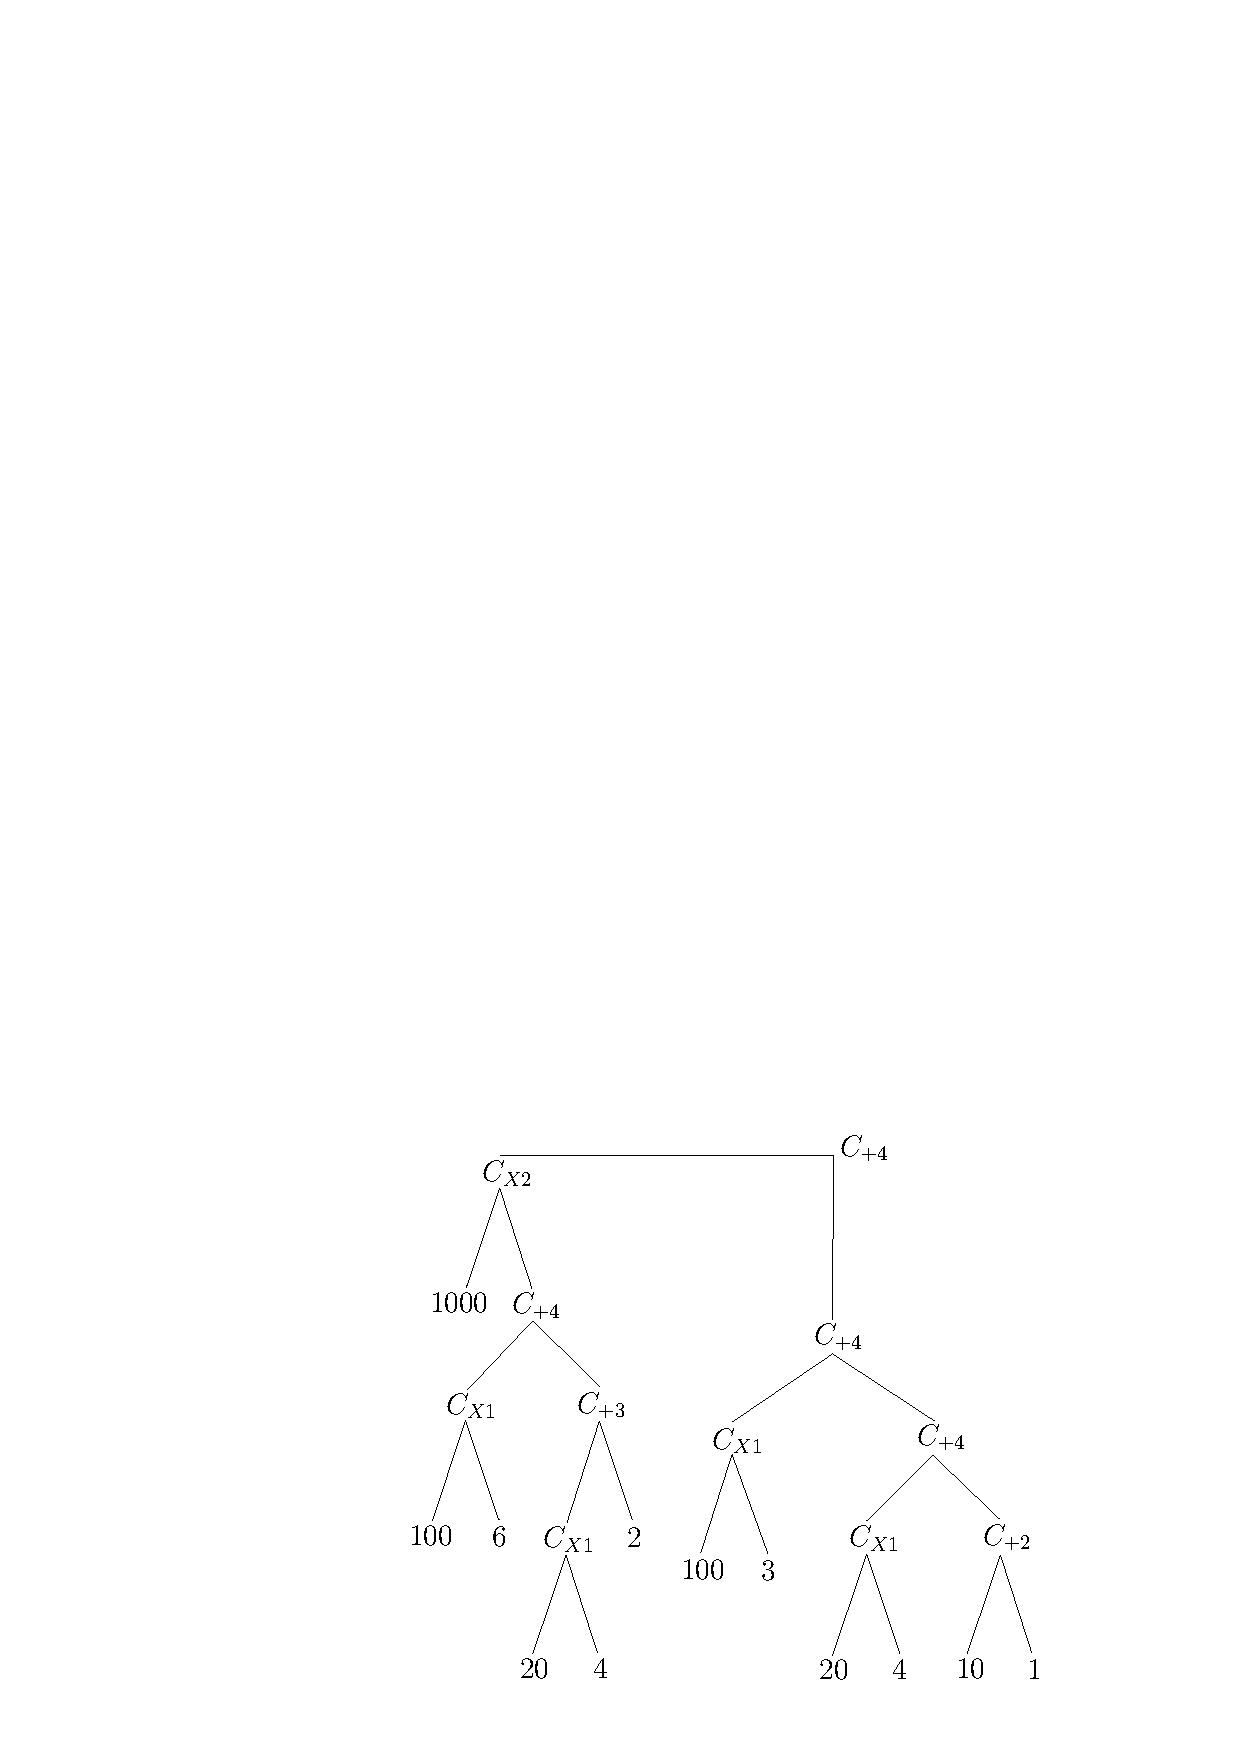
\includegraphics[width=2.8in]{Graphic/Pictures/tree-test.pdf}
 % tree-test.pdf: 595x842 pixel, 72dpi, 20.99x29.70 cm, bb=0 0 595 842
\end{center}

 \label{fig:Space-test}
\end{figure}

%  Numerals tend to be made up of combinations in which larger numerals
% precede smaller ones. Greenberg's ``efficient communication says (78-274): 
% \begin{Quote} If I express a large number, say 10,253 in the order 10,000;
%200;
% 50; 3; the very first element gives me a reasonably close approximation to the
% final result, and every successive item gives a further approximation. The
% opposite order leaves the hearer in the dark till the last item is reached.
% \end{Quote}

\clearpage

\section{Comparison and distance of Southwestern-Grusi numeral
systems}
\label{sec:NUM-dist-recons}

The goal of this section is to establish a partial Southwestern Grusi (SWG)
clustering  based on the distances each language has to others.   In comparing
the data of  the selected languages in a pairwise fashion, the distances are
calculated by assigning a numerical value to the difference/similarity  of each
pair.  The data are taken from  the cardinal numeral systems of  Chakali, Vagla,
Dɛg, Tampulma and Pasaale.\footnote{See figure \ref{fig:Gur-tree}.} These
languages are believed to be the closest to Chakali. The result of the
clustering exercise is later set against the two previous comparative linguistic
works on SWG \citep{Bend65, Mane69a, Mane69b}.

The motivation underlying the present work comes from the need for an
alternative  in comparing SWG languages.  As \citet[43]{Hegg05} write,  ``the
difficulty in applying lexicostatistics at the level of dialects rather than
distinct languages is that they generally share far `too many' cognates, even
though there may be fairly stark differences in phonetics''.  The method of the
first SWG classification  \citep{Bend65} used the `look-alike'  approach of
lexicostatistics,  a measure of linguistic similarities which takes a word as a
single data point.  

\begin{quote}
On the Swadesh first hundred Chakali is found to be closest to
Vagla with 68 look-alikes. The figures with other Grusi languages are as
follows: Tamprusi 62, Mo 61, Sisaala 47 and Kasena 39.
\end{quote}
\Source{ \cite[48]{Bend65}}

What I suggest and what seems to have become  a standard approach in
dialectology \citep{Nerb07}, is to quantify  the phonetic substance of a word in
order to exploit each word as multi-points data. An important advantage of this
approach is that one can extract substantial information from of a limited set
of words, which is a desiderata in comparing poorly documented languages
\citep{Hegg05}.  Another dimension of the approach is that I exclusively use 
data  from a single semantic domain.  The cardinal numerals were chosen for
their lack of vagueness and ambiguity (i.e. they have a strict meaning to
constituent ordering), the facility of eliciting them, the quantity of  written
works on them and their cultural and historical implications.

\subsubsection{Data}
\label{sec:NUM-data}

To my knowledge the SWG group
consists
of  Winyé, Phuie, Sissala, Western Sissala, Tumulung
Sissala, Pasaale, Chakali, Tampulma, Vagla, Dɛg and Siti  (see section
\ref{sec:INT-lit-rev}). The present
study includes only Pasaale, Chakali, Tampulma, Vagla and  Dɛg. It is quite
apparent from a limited set of data that Winyé and Phuie
show less resemblance to Chakali than the SWG languages spoken further south.
Siti is
believed to
be closely related to Vagla \citep{Klei99b} but the `recent' cardinal numeral
data needed are unavailable  at this time (available in \cite{Dela04}). The
dialects of Sissala, of which only the southmost
dialect Pasaale is included, demand a separate work. The data were collected by
the present author and are supported in
\cite{Chan09}.\footnote{\label{fot:data-orig} The Tampulma data was collected
with Yusseh
Jamani (Bowina),  Vagla   and  Dɛg with  Modesta Kanjiti (Sawla),  Vagla with
Pastor Alex Kippo  (Jang/Tuosa),  Dɛg with Kofi Mensah (New Longoro) and 
Pasaale with a UDS Wa student named Irene  (Funsi).  Earlier works which
present numerals for some of the
SWG
languages  are  \cite{Dela04, Taux21, Ratt32b, Good54}.  The data in
\cite{Chan09} are given by GILLBT or ex-GILLBT staff specialized in these
languages and myself.}

As we have seen in section \ref{sec:NUM-enum}, Chakali has  
`enumerative' numerals: these are used in counting, usually in an
increasing order
using  fingers or stones,
 and differ in form from the cardinal by (i) omitting the agreement prefix
(see
below), (ii) a tendency  to lengthen the ending vowels,  (iii)
displaying  different forms for the numbers `one' and `two', and (iv)  differ
from
the primary function of cardinal numerals in that they do not
necessarily quantify sets of entities. The selected SWG languages also have
enumerative forms with more or less the same characteristics.\footnote{The
distinction may be the source of a series of anomalies found in the literature.
For instance, when writing about  the numeral forms for 6 and 7 in Buli reported
in
\cite{Ratt32a} and \cite{Koel54}, \citeauthor{Mane75} writes that is it likely
that ``Rattray et Koelle ont appliqué la même technique: montrer deux fois trois
doigts pour `six' et trois et quatre doigts pour `sept',  et qu'ils ont obtenu
les réponses correspondantes''  \cite[183. fn130]{Mane75}.}


 Despite the belief that cardinal numerals are unequivocal items to compare,  a
normalization of the dataset  is  necessary to increase their comparability.
This avoids undesirable characteristics and  isolates the 
cardinal numeral stems. The original data appears in table
\ref{tab:NUM-SWG-card-num-data}.

\begin{table}[h]
\caption{Selected SWG cardinal numerals:  normalized
data\label{tab:data-five-swg}} 
\begin{center}
\begin{Itabular}{r|lllll}
\Hline
 & Chakali: C & Tampulma: T & Dɛg: D  & Vagla: V & Pasaala: P  \\ \hline
1 & dɪɡɪ  & diiɡɛ  &  beŋkpaŋ & kpaŋ  & kɪdɪɡɪ    \\
2 & lɪɛ  & lɛɛwa  & nɛ   &  nɛɛ & lija   \\ 
3 & toro  & toora  &  toro & horo  & to   \\ 
4 & naasɛ  & naasi &  naarɛ & naazʊ  & naa   \\ 
5 & ɲɔN  & ɲuun  & nue  & nue  & nɔŋ  \\ 
6 & loro  & nɔra  & nʊmɛl  & nʊmbɛl & dʊ   \\ 
7 & lʊpɛ  & nɔpɛ  &  nʊanɛ &  niidaanɛɛ & pɛ    \\ 
8 & ŋmɛŋtɛl  & ŋmɛnaasa  & nʊatoro  &   ŋmantannaazi & tʃori  \\ 
9 & dɪɡɪtuu  & diɡto  & nʊanaarɛ  & kabɛl  & nibi  \\ 
10 & fi  & fi  & fi & fi  & fi\\  
20 & matʃeo  & fumlɛ  &  fifraanɛ &tokko   & mɔlija  \\ 
100 & kɔwa  & kɔkwa  &  lafa & kalfa  & kɔɔ  \\ 
1000 & tʊsʊ   & tusuka  & kaɡboŋ  & kaɡboŋ  & tusi \\ 
\Hline
\end{Itabular}
\end{center}


\end{table}

The normalized data displayed in table \ref{tab:data-five-swg} differs from my
field notes and \cite{Chan09} in three ways. First,  since in many cases the
transcription of
tones is  impressionistic, I eliminate all tones. Another reason for
eliminating
tones is that tonal melodies are often associated with certain dialects.  For
instance,  one  Dɛg  consultant informed me  that {\S béŋkpóŋ} `one',  {\S
ànààrɛ̀} `four'  and   {\S ànú} `five' are associated with the Northern
dialect whereas {\S bèŋkpòŋ}, {\S ànáárɛ́} `four'  and   {\S ánʷé} with
the Southern dialect.\footnote{The main villages associated with the Northern
dialects are Bamboi, Jogboi, Teselima and  Jama, whereas New Longoro, Yara and 
Bosuoma  are associated with the Southern dialect. The transcription of tone is
available for
Chakali but is a purely impressionistic one. Further, I
gathered that there are no in-depth study of tones for any  of the SWG
languages.  I was told by many of the GILLBT staff that the late
Marjorie Crouch was an expert in Vagla tone and she could speak  the
language very well.  \cite{Crou85} is a description of the interaction of  tone,
verb and 
syllable structure in Vagla.}  Second,
the agreement prefix is removed. All the
selected languages, except for Pasaale, has an agreement slot on some of the
numerals which must be filled with either {\S a-} or {\S ba-}, depending on the
values of the plurality and humanness features of the head, as discussed
in section \ref{sec:NUM-npstruc} (e.g. in Dɛg {\S
baala banɛ} `two
men'  and {\S viine anɛ}  `two pots').  In Chakali these prefixes
attach to the numerals 2 to 7, in Vagla 2 to 7, in Dɛg 2 to 9 and in Tampulma 2
to 8.  Third,  a nasal vowel splits into a vowel followed by an abstract segment
N. This last change affects only one form in Chakali, i.e.   {\S ɲɔN} <  {\S
àɲɔ̃̀}. It is conceived that the impact of normalization would be marginal and
traceable. The original data are presented in table
\ref{tab:NUM-SWG-card-num-data} at the end of this chapter.





\subsubsection{Method}
\label{sec:NUM-method}

 %However, our method must be regarded as a lightweight one.
The method  proposed, i.e. phonetic comparison,  is insprired by
\cite{Hegg05, McMa06, Tedl07}. The idea behind phonetic comparison is to produce
finer-grained measurements when lexical comparison limit the number of data
points. However, compared to the work referred to above, the method used
here must be
regarded as lightweight: as the reader will realize, the ``phonetics'' is
very primitive and  the alignment is handmade.\footnote{This work is a
pen-and-paper application. For a computational
implementation, see \cite{Conv96} among others, and for a review of
computational alignment methods, see  \cite{Kond02}.} Yet I consider
these issues more as  (future) refinements than
methodological flaws.  Let us see step by step how I calculate the distances
between the selected languages and how I arrive at a SWG clustering.

%When one compare cognate words one always makes sure that the words can be
%aligned. Thus comparing the lexical forms precedes the alignment.

 The first step is to align the strings. By {\it alignment} I mean
matching the phonetic segments in a way which  minimizes the difference between
two
words.  This is shown in figure
\ref{fig:NUM-align-quant-two-EXE}a. The second step is to calculate the distance
between two languages. Difference is costly, that is,  the more two languages
are dissimilar, the higher the value.  The difference between two languages is
quantified by assigning a substitution cost to a type of difference. The costs
are shown in table \ref{tab:cod-sys}. For instance, if there is a single
consonant mismatch between two words,  e.g. `three'  Vagla {\S horo} vs. Dɛg {\S
toro}, the cost is 1.   The relative costs are linguistically motivated: for
instance, a common observation is that vowels are usually less stable than
consonants across dialects and language stages. Nonetheless this is surely the
crudest substitution cost one can design.\footnote{The cost of the difference
{\F [p]}/{\F [r]} is the same as the cost of  {\F [s]}/{\F [z]}. See
\cite{Heer02, Kond03} for an overview of methods for  weighting phonetic
differences.} 

\begin{table}[h!]
\caption{Substitution costs \label{tab:cod-sys}} 

\centering
% use packages: array
\begin{tabular}{ll}
 Difference & Cost \\ \hline 
Exact match& 0 \\ 
(V)owel mismatch & 0.5 \\ 
(C)onsonant mismatch & 1 \\ 
Gap (i.e -) mismatch due to vowel lenght & 0.5\\
Gap (i.e -) mismatch with C or V & 1\\
 
      \end{tabular}

      \end{table}

Then a {\it distance matrix} is constructed based on the numerical distance
between   words taken pairwise.  As an illustration,  in table
\ref{fig:NUM-align-quant-two-EXE}b  the
distance matrix
gathers the total distances of each language pair for the word `two'.  If we
take the distance between Tampulma and Vagla as an example, we see that 3 is the
sum of three substitution costs each worth 1: one consonant mismatch, i.e. {\S
l} vs. {\S n}, and two gap mismatches, i.e.   {\S w} vs. {\S -} and {\S a} vs.
{\S -}. The last step is to cluster the languages according to the value
displayed on the distance matrix. The {\it dendrogram} in figure
\ref{fig:NUM-align-quant-two-EXE}c illustrates the arrangement of the clusters
produced by the distance matrix. 


\begin{figure}[h!]

 \centering
 \subfloat[][Alignment]{{\I 
\begin{tabular}{l|lllll}
C & l & ɪ & ɛ & - & -\\
T & l & ɛ & ɛ & w & a\\
D &  n & ɛ & - & - & -\\
V &  n & ɛ & ɛ & - & -\\
P & l & i & - & j & a\\
\end{tabular}}} 
\qquad
\subfloat[][Distance matrix]{
\begin{tabular}{l|lllll}
  & C & T & D & V & P \\ \hline
C & - & 2.5 & 2 & 1.5 & 3\\
T &   &-    &  3.5  & 3 & 2\\
D &   &	    &  -  & 0.5	& 3.5\\
V &&&&-&4\\
P &&&&&-\\

\end{tabular}}

\subfloat[][Dendrogram]{
 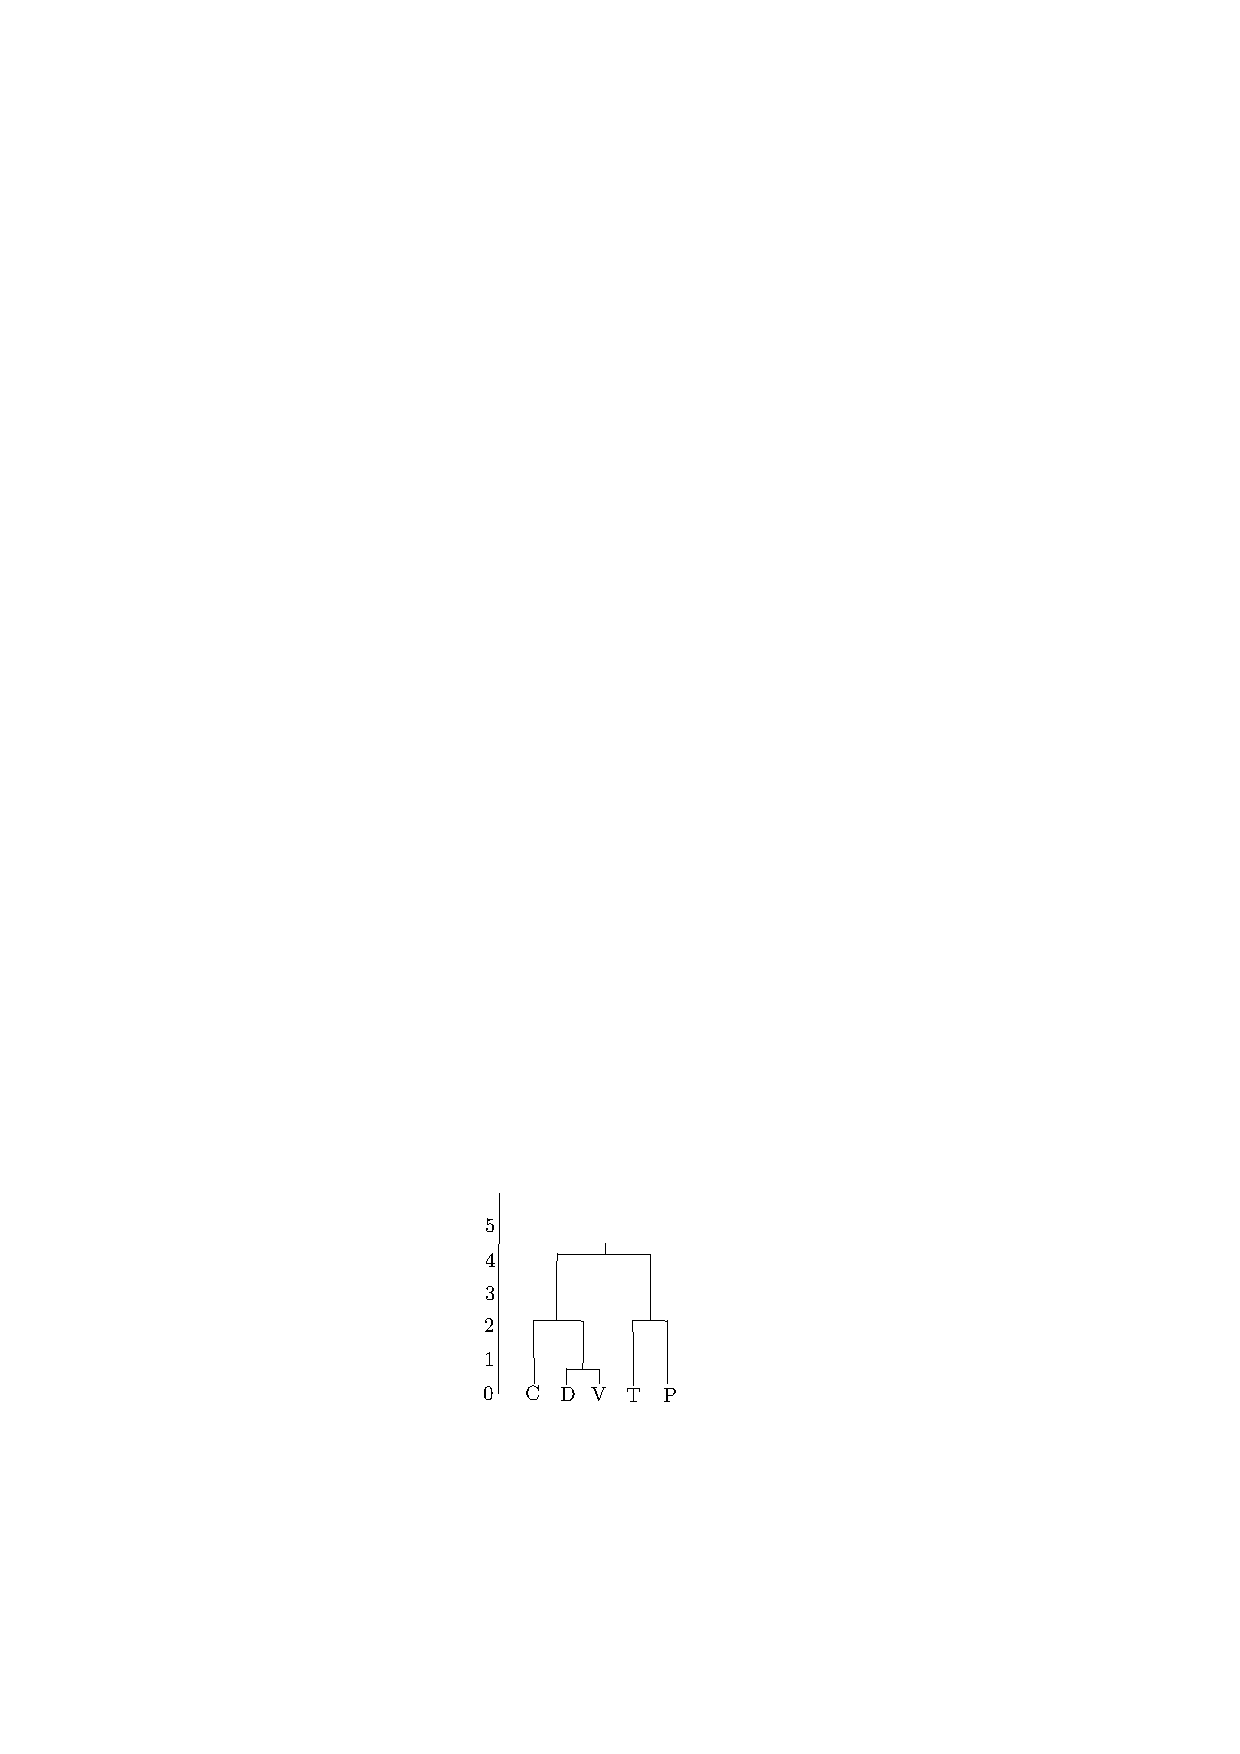
\includegraphics[width=6cm,height=3.8cm]{Graphic/Pictures/tree-2.pdf}
}
 
% tree-2.pdf: 595x842 pixel, 72dpi, 20.99x29.70 cm, bb=0 0 595 84

\caption[Clustering   Chakali, Tampulma,  Dɛg, Vagla and  Pasaale 
for the
expressions  `two']{Clustering  C: Chakali, T: Tampulma, D: Dɛg, V: Vagla and P:
Pasaale 
for the
expressions  `two'\label{fig:NUM-align-quant-two-EXE}}
\end{figure}






The clustering develops in phases and starts
with the lowest value. Consequently  Dɛg and Vagla are clustered at the initial
stage (value 0.5); they are the closest pair of languages.   If  the next lowest
value clusters two languages of which one is already in a cluster created at a
previous stage, the language not yet clustered is merged at the highest value of
its pairing with each language, i.e. the maximum cost.  In this way, the second
phase
merges Tampulma and Pasaale (value 2)  followed by a third phase bringing
Chakali with the cluster Dɛg-Vagla at value
2,  since Chakali and Vagla
are at a distance of 2 whereas Chakali and Dɛg are at a distance of 1.5.  The
last phase gathers the
cluster Tampulma-Pasaale and the cluster Chakali-[Dɛg-Vagla]  (value 4).




The dendrogram illustrates that, given the current dataset,  the cluster Vagla
and
Dɛg are the closest languages, followed by the cluster  Tampulma and Pasaale.
Chakali is closer to the cluster Dɛg-Vagla (max. cost 2) than to the cluster
Tampulma-Pasaale  (max. cost 3). Of course the clustering result is not
representative or conclusive  as it  is based on a single word per language.
The goal here is to apply the same procedure to all atomic numerals in the five
languages. 

A word of caution is in order. In practice comparativists  carefully  avoid
words believed to be of non-genetic origin. In the present
case I do not attempt to identify loans since I am  interested in
establishing a SWG clustering in synchrony and I do so  based on the entire
lexicalisation of a 
single semantic domain.  The
only criterion I suggest  for
comparing a  numeral is that at least three languages
align (>50\%).  Only indirectly may  this criterion identify cognate items
and loans, something I will consider in section \ref{sec:NUM-compar-discuss}. 


\subsection{Clustering results}
\label{sec:clustres1}


A comparison presupposes that the forms are indeed `comparable'. In applying
the method designed in section \ref{sec:NUM-method}, a division between the set
of forms \{2,3,4,5,10\} and the set
\{1,6,7,100,1000\} emerge. This division originates from the success or failure 
to align. The former set represents cases where all five numeral
forms align.
For  the latter set, there is a clear separation between a group consisting
of Chakali, Pasaale and Tampulma and a group consisting of Vagla and Dɛg. Table
\ref{tab:NUM-SWG-sets-sample} displays for each number the result of all pairs.

\begin{table}[htb]
\centering
\caption[Distances of numeral sets  \{2,3,4,5,10\} and  
\{1,6,7,100,1000\}]{Distances of numeral sets  \{2,3,4,5,10\} and  
\{1,6,7,100,1000\}. C: Chakali, T: Tampulma,
D: Dɛg, V: Vagla and
P: Pasaale. \label{tab:NUM-SWG-sets-sample}}

\subfloat[][ \{2,3,4,5,10\}]{
\begin{Itabular}{lllllllllll}
 \Hline
 & CT & CD & CV & CP & TD & TV & TP & DV & DP & VP \\[1ex] \hline
two & 2.5 & 2 & 1.5 & 3 & 3.5 & 3 & 2 & 0.5 & 3.5 & 4 \\ 
three & 1 & 0 & 1 & 2 & 1 & 2 & 2.5 & 1 & 2 & 3 \\ 
four & 0.5 & 1 & 1.5 & 2 & 1.5 & 1.5 & 2 & 1.5 & 2 & 2 \\ 
five & 2 & 3 & 3 & 2 & 2.5 & 2.5 & 3 & 0 & 2 & 2 \\ 
ten & 0 & 0 & 0 & 0 & 0 & 0 & 0 & 0 & 0 & 0 \\[2ex] \hline
\textsc{sum} & 6 & 6 & 7 & 9 & 8.5 & 9 & 9.5 & 3 & 9.5 & 11 \\ 
 \Hline
\end{Itabular}}

\subfloat[][\{1,6,7,100,1000\}]{
 \begin{Itabular}{lllll}

 \Hline
 & CT & CP & TP & DV \\[1ex] \hline
one & 1.5 & 2 & 3.5 & 3 \\ 
six & 2 & 3.5 & 3.5 & 1 \\ 
seven & 1.5 & 2 & 2 & 3.5 \\ 
hundred & 1 & 2.5 & 3.5 & 3 \\ 
thousand & 3 & 1 & 2.5 & 0 \\[2ex] \hline
 
\textsc{sum} & 9 & 11 & 15 & 10.5 \\ 
\Hline
\end{Itabular}}
\end{table}


The sum value associated with each pair in table \ref{tab:NUM-SWG-sets-sample}
appears in the distance matrices of figure
\ref{fig:NUM-align-quant-grand}.  From these values, two  dendrograms are
built
for the set 
\{2,3,4,5,10\} and the set \{1,6,7,100,1000\}. They represent respectively 
the clusterings
labeled SWG, and what I call Northern Southwestern Grusi
(NSWG).  A  division NSWG and South Southwestern Grusi (SSWG) is created as a
consequence of a failure to align for the set \{1,6,7,100,1000\}, e.g. `one'
 [C: {\S dɪɡɪ},   T: {\S  diiɡɛ} and P: {\S kɪdɪɡɪ}] vs.    [D: {\S  beŋkpaŋ}
and
 V:
{\S kpaŋ}].   The dendrogram for SSWG is not displayed but the pair
Dɛg-Vagla has a distance of 10.5 for the set \{1,6,7,100,1000\}. Moreover, the
clustering of the set \{2,3,4,5,10\} alone tells us that the division NSWG and
SSWG is indeed present. The pair Dɛg-Vagla has the lowest value in table
\ref{tab:NUM-SWG-sets-sample}a. This indicates that among the ten pairing
possibilities, the two languages have the least differences. 



\begin{figure}[htb]

\centering

 \subfloat[][Distance matrix SWG]{ 
\begin{tabular}{l|llllll}
 & C & T & D & V & P \\ \hline
C & - & 6 & 6 & 7 & 9  \\ 
T &  & - & 8.5 & 9  & 9.5 \\ 
D &  &  &  -&  3& 9.5 \\ 
V &  &  &  & - & 11 \\ 
P &  &  &  &  &-  \\ 
\end{tabular}} 
\qquad
\subfloat[][Distance matrix NSWG]{
\begin{tabular}{l|llp{0.6cm}l}
 & C & T & P \\ \hline
C & - & 9 & 11  \\ 
T &  &  -&  15\\ 
P &  &  &-  \\ 
\end{tabular}}
\qquad
\subfloat[][SGW
Dendrogram]{
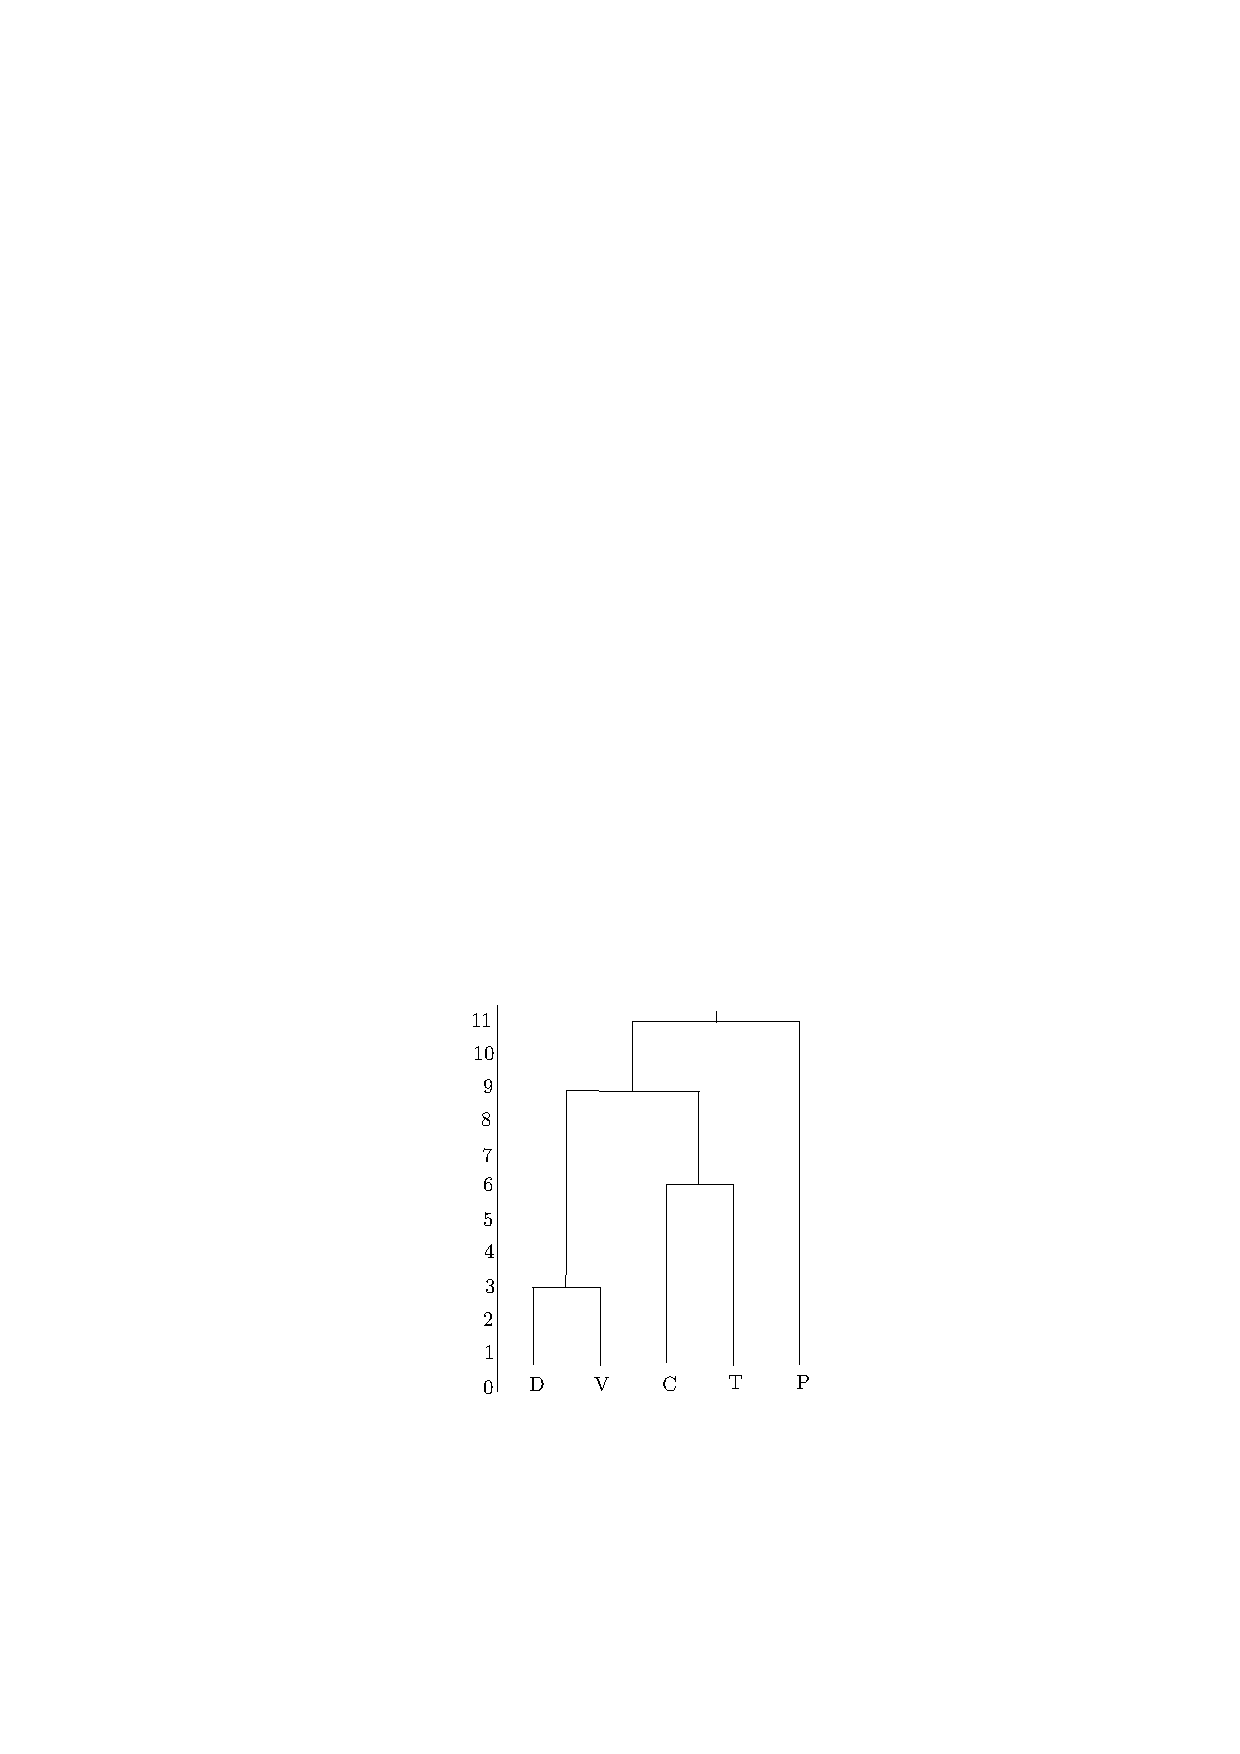
\includegraphics[width=5cm,height=5.5cm]{Graphic/Pictures/TGM-A-E.pdf}
}
\qquad
\subfloat[][NSWG
Dendrogram]{
 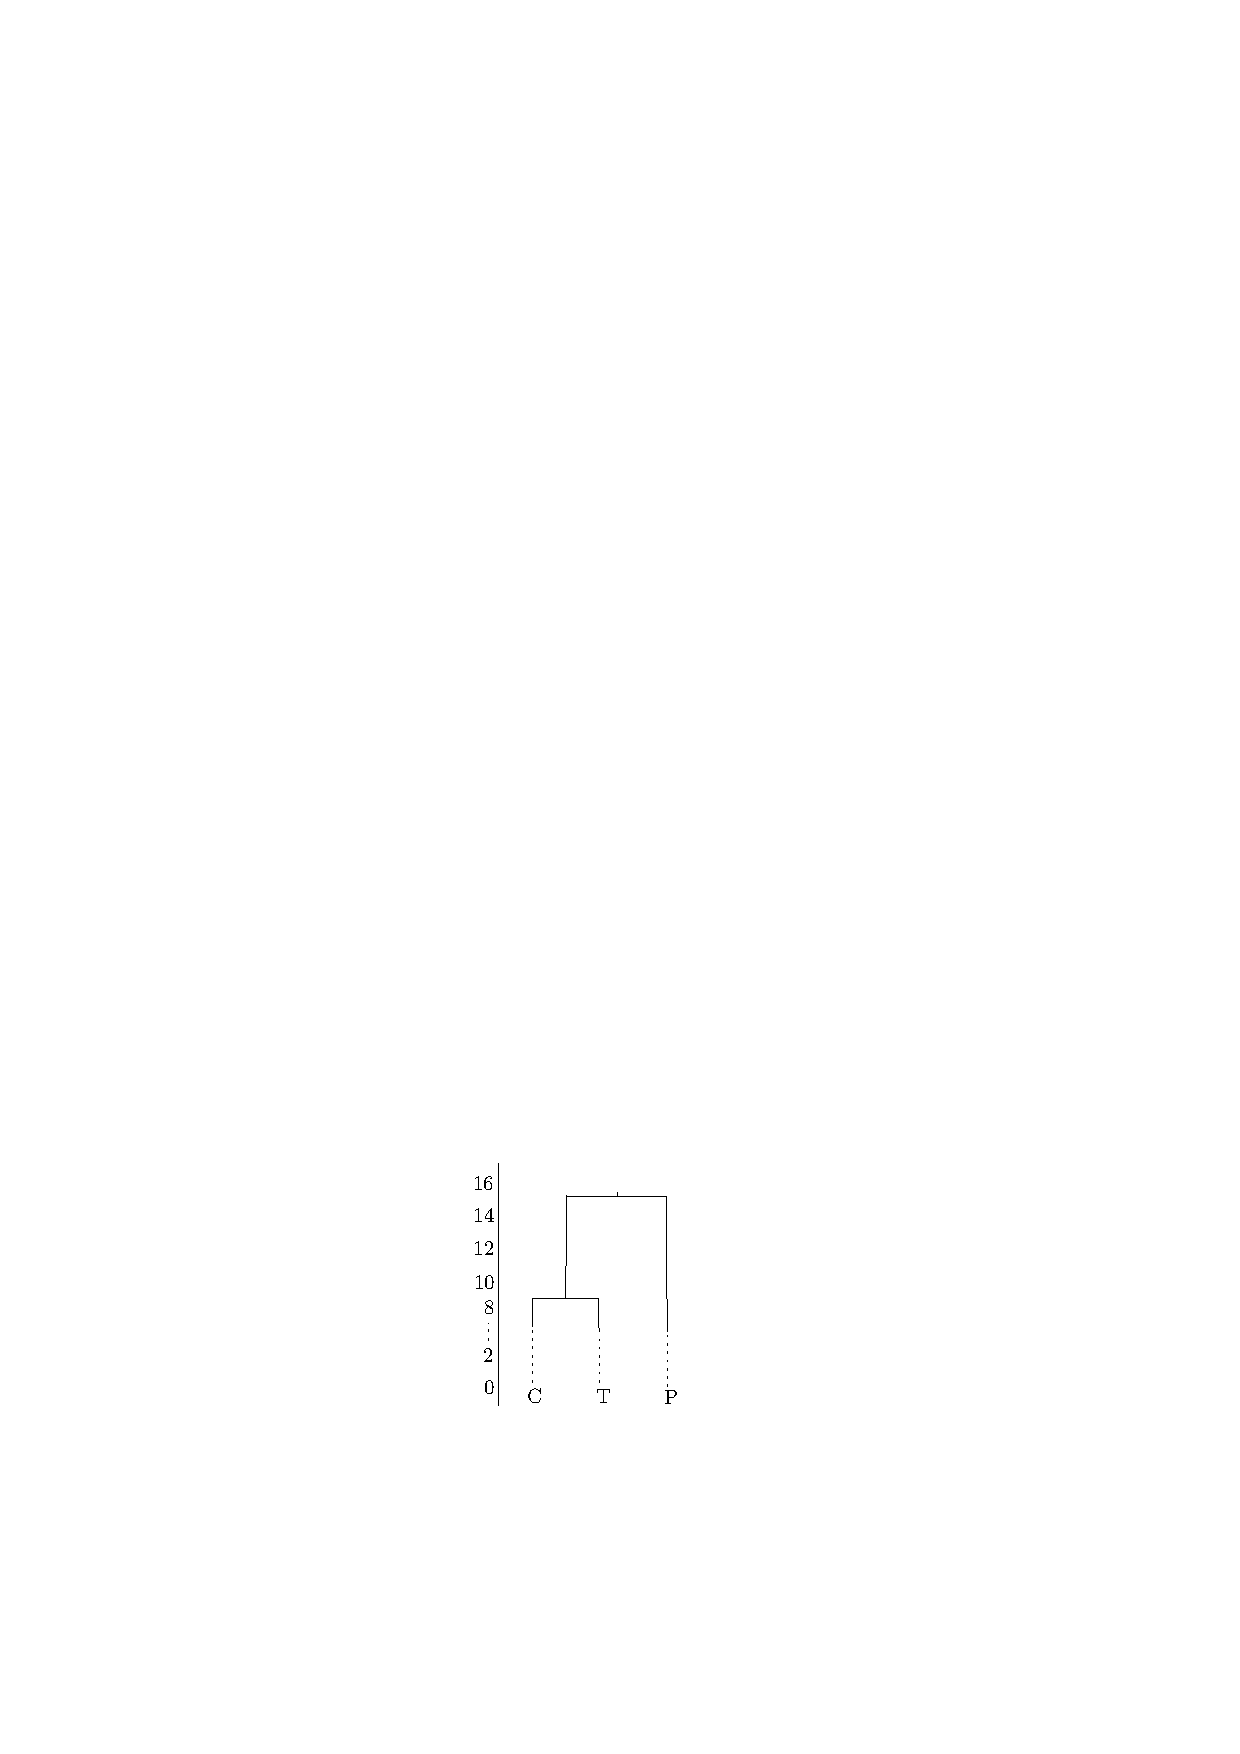
\includegraphics[width=5cm,height=3.5cm]{Graphic/Pictures/TGM-ABE.pdf}
}

\caption[Grand matrix and dendrogram for SWG  and NSWG]{Grand matrix and
dendrogram for SWG \{C, T, D, V, P\} and NSWG
\{C, T, P\}  \label{fig:NUM-align-quant-grand}}
\end{figure}


In figure \ref{fig:NUM-align-quant-grand}c,  the SWG  dendrogram shows that  
Dɛg
and Vagla are clustered at
initial stage (value 3), then Chakali and Tampulma are clustered together in the
second phase (value 6). The cluster  Dɛg-Vagla and the cluster
Chakali-Tampulma
are clustered in a third phase (value 9), and finally, Pasaale
is clustered in
the
big family (value 11).  In figure  \ref{fig:NUM-align-quant-grand}d, the NSWG 
dendrogram shows that Chakali and
Tampulma clusters at initial stage (value 9) and that Pasaale  clusters with
the Chakali-Tampulma cluster on a second and last phase (value 15).

On the whole, the  clusters  [D-V] and [C-T-P]  appear repeatedly.  In the next
section,  these clusters will resurge when we look at the morphosyntactic 
characteristics of the languages. 

% ducielii and kɔsa is pluralKow is the singular and kousi or kɔwa is the
%plural.
% Tusu is the singular and tusa is the plural eg. tusa lia is 2000. u can't say
% tusu lia. Yeah machiu is used throughout. There is no variation.

\subsubsection{Operator and morphosyntax}
\label{sec:NUM-oper-morpho}


In the previous section, I compared   the phonetic characteristics of the
atomic cardinal numerals of the five languages.  Let us now turn to their
morphosyntactic characteristics and see whether they corroborate the clustering 
presented in table \ref{fig:NUM-align-quant-grand}.  Comparing morphosyntactic 
characteristics will give us the possibility of clustering expressions in
languages which differ lexically, and therefore have no access to segmental
comparison. Among others, the case of number 9 in some SWG languages is one
where segmental comparison is impracticable, but
morphosyntactic comparison indeed indicates similarities among three languages.

The discussion employs the terminology introduced in section
\ref{sec:NUM-gramarith};  a simple lexemic representation is an atomic numeral
(i.e. {\W a}),  a base is a serialized atom (i.e.  {\W b}) and  a non-lexemic
representation containing morphemes and arithmetical operations is called a
complex numeral (i.e.  {\W C}).  Symbols within parenthesis represent covert
expressions. Consider table \ref{tab:NUMmorphsyn1-10}.


\begin{table}[h]
 \caption{Morphosyntactic characteristics of  series  [1-10]
\label{tab:NUMmorphsyn1-10}}
 
 \centering
%\Hline 

\subfloat[][C: Chakali]{\footnotesize
\begin{tabular}{p{0.5cm}l}


1 & {\Y a}\\ 
2 & {\Y a}\\ 
3 & {\Y a}\\
4 & {\Y a}\\
5 & {\Y a}\\
6 & {\Y a}\\
7 & {\Y a}\\
8 & {\Y a}\\
9 &  {\Y (b)}-{\Y a}\\
10 & {\Y a}\\


\end{tabular}
} 
\quad
\subfloat[][T: Tampulma]{\footnotesize
\begin{tabular}{p{0.6cm}l}


1 & {\Y a}\\ 
2 & {\Y a}\\ 
3 & {\Y a}\\
4 & {\Y a}\\
5 & {\Y a}\\
6 & {\Y a}\\
7 & {\Y a}\\
8 & {\Y a}\\
9 &  {\Y (b)}-{\Y a}\\
10 & {\Y a}\\


\end{tabular}
} 
\quad
\subfloat[][D: Dɛg]{\footnotesize
\begin{tabular}{p{0.4cm}l}



1 & {\Y a}\\ 
2 & {\Y a}\\ 
3 & {\Y a}\\
4 & {\Y a}\\
5 & {\Y a}\\
6 & {\Y b}(+){\Y a}\\
7 & {\Y b}(+){\Y a}\\
8 & {\Y b}(+){\Y a}\\
9 & {\Y b}(+){\Y a}\\
10 & {\Y a}\\


\end{tabular}
} 
\quad
\subfloat[][V: Vagla]{\footnotesize
\begin{tabular}{p{0.5cm}l}



1 & {\Y a}\\ 
2 & {\Y a}\\ 
3 & {\Y a}\\
4 & {\Y a}\\
5 & {\Y a}\\
6 & {\Y b}(+){\Y a}\\
7 & {\Y (b)}(+){\Y a}\\
8 & {\Y a}\\
9 &  {\Y (b)}-{\Y a}\\
10 & {\Y a}\\


\end{tabular}
} 
\quad
\subfloat[][P: Pasaale]{\footnotesize
\begin{tabular}{p{0.5cm}l}

1 & {\Y a}\\ 
2 & {\Y a}\\ 
3 & {\Y a}\\
4 & {\Y a}\\
5 & {\Y a}\\
6 & {\Y a}\\
7 & {\Y a}\\
8 & {\Y a}\\
9 &  {\Y a}\\
10 & {\Y a}\\


\end{tabular}
} 

%\Hline

\end{table}


  


In table \ref{tab:NUMmorphsyn1-10}, Chakali  and Tampulma   are identical; the
series [1-10] is made up of atoms except for 9 which is a complex expression, a
subtraction in which the minuend is covert. If we were to ignore the expression
for 9, Pasaale   would be identical to Chakali and Tampulma. Dɛg displays a
`complete' base-5 system, i.e. 5 is serialized completely. Dɛg's [6-9] and
Vagla's [6-7] are the only  expressions using 5 as augend. Vagla resembles Dɛg
except for the number `eight' and `nine'.  In Vagla, 5 is serialized only
partially; 8 is expressed with an atom and 9 with subtraction in which the
minuend is covert. All the languages have the atomic numeral {\S fi} to
designate the number 10.  In fact, Dɛg displays a `nearly complete' base-5
system since  the atomic numeral {\S fi} is used to express 10 instead of a
potential complex {\W b}_{5}+{\W a}_{5}.






\begin{table}[ǃh]
\caption{Morphosyntactic characteristics of series  [11-19] 
\label{tab:NUMmorphsyn11-19}}

 \centering
\begin{tabular}{lllll}
\Hline
  C: Chakali &	T: Tampulma &  D: Dɛg & V: Vagla & P: Pasaale \\[1ex]
\hline

 {\Y b}_{10}+{\Y a}_{[1-8]} & {\Y  b}_{10}+{\Y a}_{[1-8]} &   {\Y b}_{10}+{\Y
C}_{[6-9]} & {\Y b}_{10}+{\Y C}_{[6,7,9]}  & {\Y b}_{10}+{\Y a}_{[1-9]} \\

    {\Y b}_{10}+{\Y C}_{9}        &        {\Y b}_{10}+{\Y C}_{9}   
      &  {\Y b}_{10}+{\Y a}_{[1-5]}       &  {\Y b}_{10}+{\Y a}_{[1-5, 8]}    &
\\
 
\Hline

\end{tabular} 
 
\end{table}


Table \ref{tab:NUMmorphsyn11-19} displays the relevant characteristics  of
the complex numerals expressing the progression 11 to 19.  The five languages
use  10 as a base, followed in turn by an overt adding operator and 
their respective expressions of the series [1-9]. All of them,  except
Pasaale, have a form {\S dV} as operator, i.e. C {\S dɪ}, T  {\S di}, D
{\S dɛ}
and V {\S dɪ}. 






\begin{table}[htb]

 \caption{Morphosyntactic characteristics for series  [21-99]}
 \label{tab:NUMmorphsyn21-99}
 \centering
 
% use packages: array
\begin{tabular}{l|llll} 
\Hline
 & 30  & 40  & 50  & 80  \\
\hline  
C:  & 20$+$10 & 20$\cdot$2  & [20$\cdot$2]$+$10 &  20$\cdot$4 \\ 
T:   & 10.{\sc pl}$\cdot$3   & 10.{\sc pl}$\cdot$4 & 10.{\sc pl}$\cdot$5 & 
10.{\sc pl}$\cdot$8 \\ 
D:  & 10.{\sc pl}$\cdot$3 &  10.{\sc pl}$\cdot$4 &  10.{\sc pl}$\cdot$5&
10.{\sc pl}$\cdot$8  \\ 
 V:  & 20$+$10 &   20$\cdot$2&  [20$\cdot$2]$+$10 &  20$\cdot$4 \\ 
P:  & 20$+$10 &   20$\cdot$2& [20$\cdot$2]$+$10 & 20$\cdot$4 \\ 
\Hline
 \end{tabular}


\end{table}

In table \ref{tab:NUMmorphsyn21-99},  the morphosyntactic characteristics of the
 complex expressions for the progression  21 to 99 are displayed.   A clear
division appears between a group consisting of Tampulma and Dɛg  and a group
consisting of Chakali, Vagla and Pasaale. The former group is  base-10 (decimal)
and the latter base-20 (vigesimal).  

Further, in each language,  the two series 11-19 and
21-99 may involve the same or a different adding operator.   Tampulma, Dɛg
and Pasaale use the same adding operator (i.e. T: {\S dV}, D: {\S dɛ} and 
P: {\S bee}) for the two series, whereas Chakali and Vagla use a different
adding operator for the series [11-19]/[21-99] which cannot be triggered solely
by  phonological context (i.e. C: {\S d}V/{\S anɪ} and V: {\S d}V/{\S
nɪ}).  Finally, multiplication  is not phonetically expressed 
and the series involving hundreds and thousands are decimal in all languages. 
Let us now summarize and examine whether the phonetic and morphosyntactic 
characteristics of the numerals confirm a particular clustering.


The cluster Vagla-Dɛg (SSWG)  is sustained in the number series  [1-10]. Only
these two  languages have base-5 systems.  Further, contrary to the overall
expression of addition, the adding operator is covert.   The cluster
Chakali-Tampulma-Pasaale  (NSWG) is mainly atomic for the same series. For the
number 9, the subtraction operation cuts across  NSWG  and SSWG:  Vagla ,
Tampulma and Chakali  use subtraction of  type `one remains'.  Nonetheless three
characteristics maintain the split. First,  the forms for `one' in Chakali and
Tampulma are the same as those expressing `one' in complex expressions, i.e. {\S
dɪɡɪ} and  {\S diɡ} (< {\S diigɛ}) respectively. In Vagla, {\S bɛl} is used in
complex expression instead of {\S kpaŋ}.\footnote{For Dɛg  {\F beŋkpaŋ},  I
assume that the first morpheme is also {\F bɛl} (>  {\F beŋ}), and that the
velar nasal is the result of homorganic change {/l/}  $>$ {/ŋ/} caused by
the labio-velar {/kp/} of {\F kpaŋ}. The form {\F bɛl} is found in the
formation of other numerals in both  Dɛg and Vagla (e.g.  vag: {\F bɛl} `one',
{\F anue} `five', {\F anu-m-bɛl} `six': {\F ka} `leave, be left' {\F kabɛl}
`left one'  (=  10 - 1). In Dɛg {\F kpaŋkpaŋa}, which appears to be a plural
form for `one', means `one by one' or an iteration of oneness, e.g.  {\F Kuari a
kuna maa di ra dauri kpaŋkpaŋa} `Get all the things and lay them down one by
one' (Dɛg lexicon,  Tony Naden p.c.).} Second, the order of `one' and `remain'
is reversed, i.e.  Tampulma {\S diɡ-to} and Chakali  {\S dɪɡɪ-tuu} are analysed
as `one-absent' and Vagla {\S  kabɛl} is analysed as  `absent-one'. And third,
the existence of {\S sandoso} in Tampulma \citep{Ratt32b, Good54} and Chakali
strengthens a cluster NSWG  and SSWG. For the series [11-19] all languages use a
base-10 complex expressions with overt adding operators and the addend  is their
respective [1-9] series.   The division NSWG and SSWG gets blurred in the series
[21-99]. There we find for the first time that the languages Dɛg and Tampulma
share a common characteristic which is not found in the other languages (i.e.
base-10 in the series [21-99]).  Chakali, Pasaale and Vagla are base-20. 


The few cases of suppletion are important to mention. `One' has two  forms in
Tampulma; a form for the number 1 and another form in the expressions
designating the numbers 11, 21, 31, (...), 91. Similarly, `one' has two  forms
in Dɛg and Vagla; a form for 1 and another form
in the formation of 6 in Dɛg, and 6 and 9 in Vagla. Finally, Vagla has a free
variant atom for 50, which is probably borrowed from Gonja, and 10 is
suppletive only in the expression for 30. 


Whether comparing phonetic and morphosyntactic characteristics  strengthens or
weakens the clusters NSWG and SSWG is unclear. On the one hand, the bases
involved in
the series [21-99] cut across the division established. On the other hand, the
division is confirmed by the languages' characteristic for the series  [1-10].
For the most part, Vagla and Dɛg belong to a cluster which uses 5 as a base,
whereas Chakali, Tampulma and Pasaale belong to a cluster whose progression from
1 to 10 is expressed with atomic expressions. 

Below I examine the method and result by looking for correlations between the
cluster derived from the phonetic comparison and those derived from
lexicostatistics and the comparative method. Next,  the result of
phonetic comparison applied to cardinal numerals are compared with the result of
another
semantic domain.



\paragraph{\cite{Bend65}}
\label{sec:NUM-bend65}

 The clustering found in  \citet[50]{Bend65} is reproduced in figure
\ref{fig:Bend-clust}. 

 \begin{figure}[htbp]
 \centering
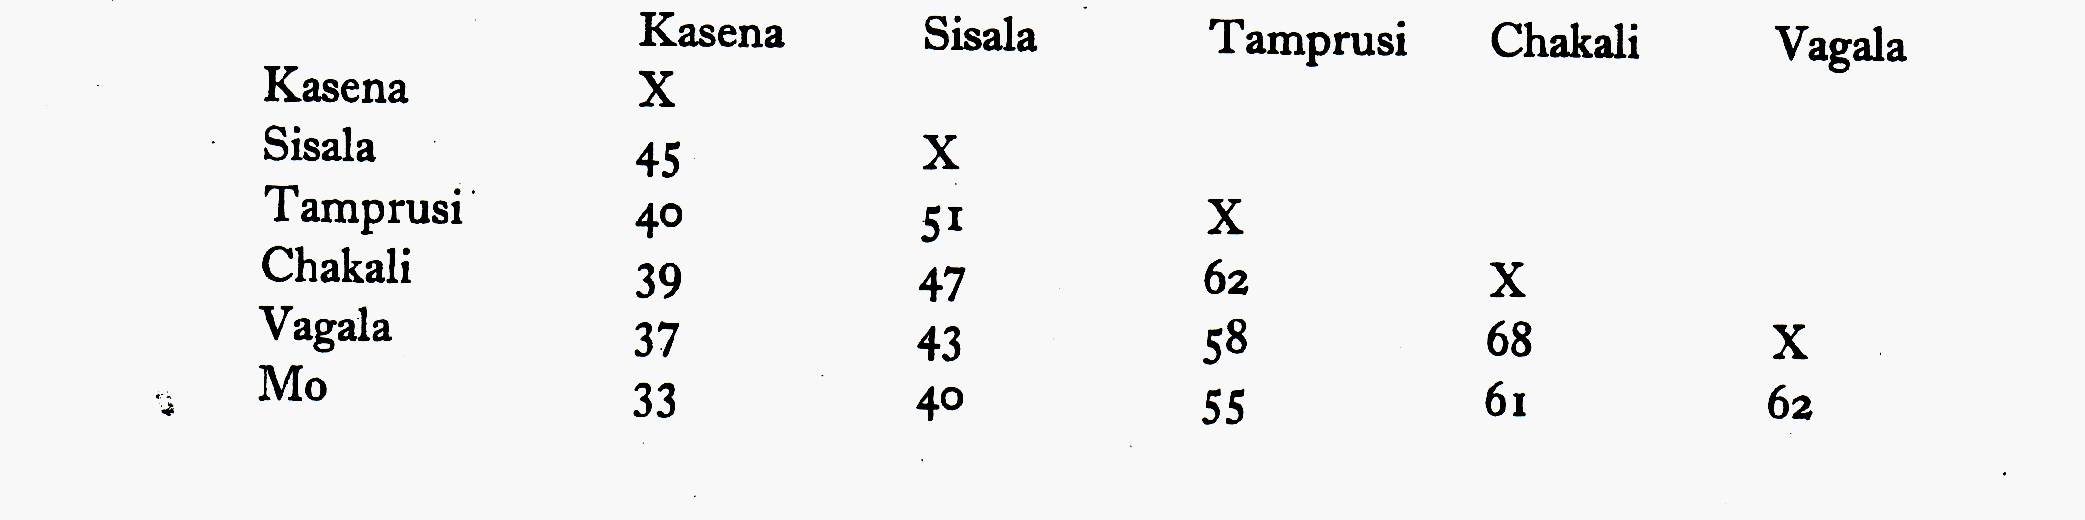
\includegraphics[width=10cm,height=3cm]{Graphic/Pictures/File-0001-page.jpg}
\caption{Clustering of \citet[50]{Bend65} \label{fig:Bend-clust}}
\end{figure}

To begin with, I cannot use Pasaale to compare the clusterings since
\citeauthor{Bend65} does not
specify which Sisaala dialects
he uses.\footnote{Bendor-Samuel
acknowledges Mr. E. R. Rowland for the collection of the Chakali and Sisaala
data. It was impossible for me to trace back  the source locations, the
consultants or the original manuscripts.
To my knowledge `Sisaala'
is  divided into four dialects \citep{Lewi09}, some of them mutually
unintelligible.  Folk linguistics make
even
more finer distinctions,  so `Sisaala'  should be treated with prudence.}
Still, 
his lexicostatistics' result
indicates that Vagla and Chakali are the closest pair of languages (68/97),
followed by both the pairs Tampulma-Chakali (62/97) and the Dɛg-Vagla (62/97).
The
latter two pairs are the closest clusters in  figure
\ref{fig:NUM-align-quant-grand}.



\paragraph{\cite{Mane69a}}
\label{sec:NUM-mane69a}

For the languages
at hand,  \citeauthor{Mane69a} mainly adopts Bendor-Samuel's data. In 
\citet[16-18]{Mane69a}, he uses exclusively the Chakali data offered in
\cite{Bend65},  for
Dɛg he uses
\cite{Dela04} (i.e. {\it degha}) and \cite{Bend65} (i.e. {\it mo}), for Vagla he
uses
\cite{Ratt32a, Crou66, Bend65} and for Tampulma he uses   \cite{Ratt32a,
Bend65}. However, the possibility for Manessy to design a SWG clustering
originates from his exceptional skill in working with the traditional
comparative method. The tree in figure \ref{fig:Mane-clust} is the result of his
detailed  analysis of phonetic and
morphological correspondances.\footnote{In figure  \ref{fig:Mane-clust},
the letters A, B and C represents Manessy's division of {\it gurunsi},
corresponding respectively to the Northern, Eastern and  Western of 
\cite{Nade89}. The
language {\it gouressi}, which Manessy adopts from \cite{Dela04}, is probably a
dialect of Sisaala. The languages {\it mo} and {\it degha} are both known 
today as Dɛg. }



 \begin{figure}[htb]
 \centering
 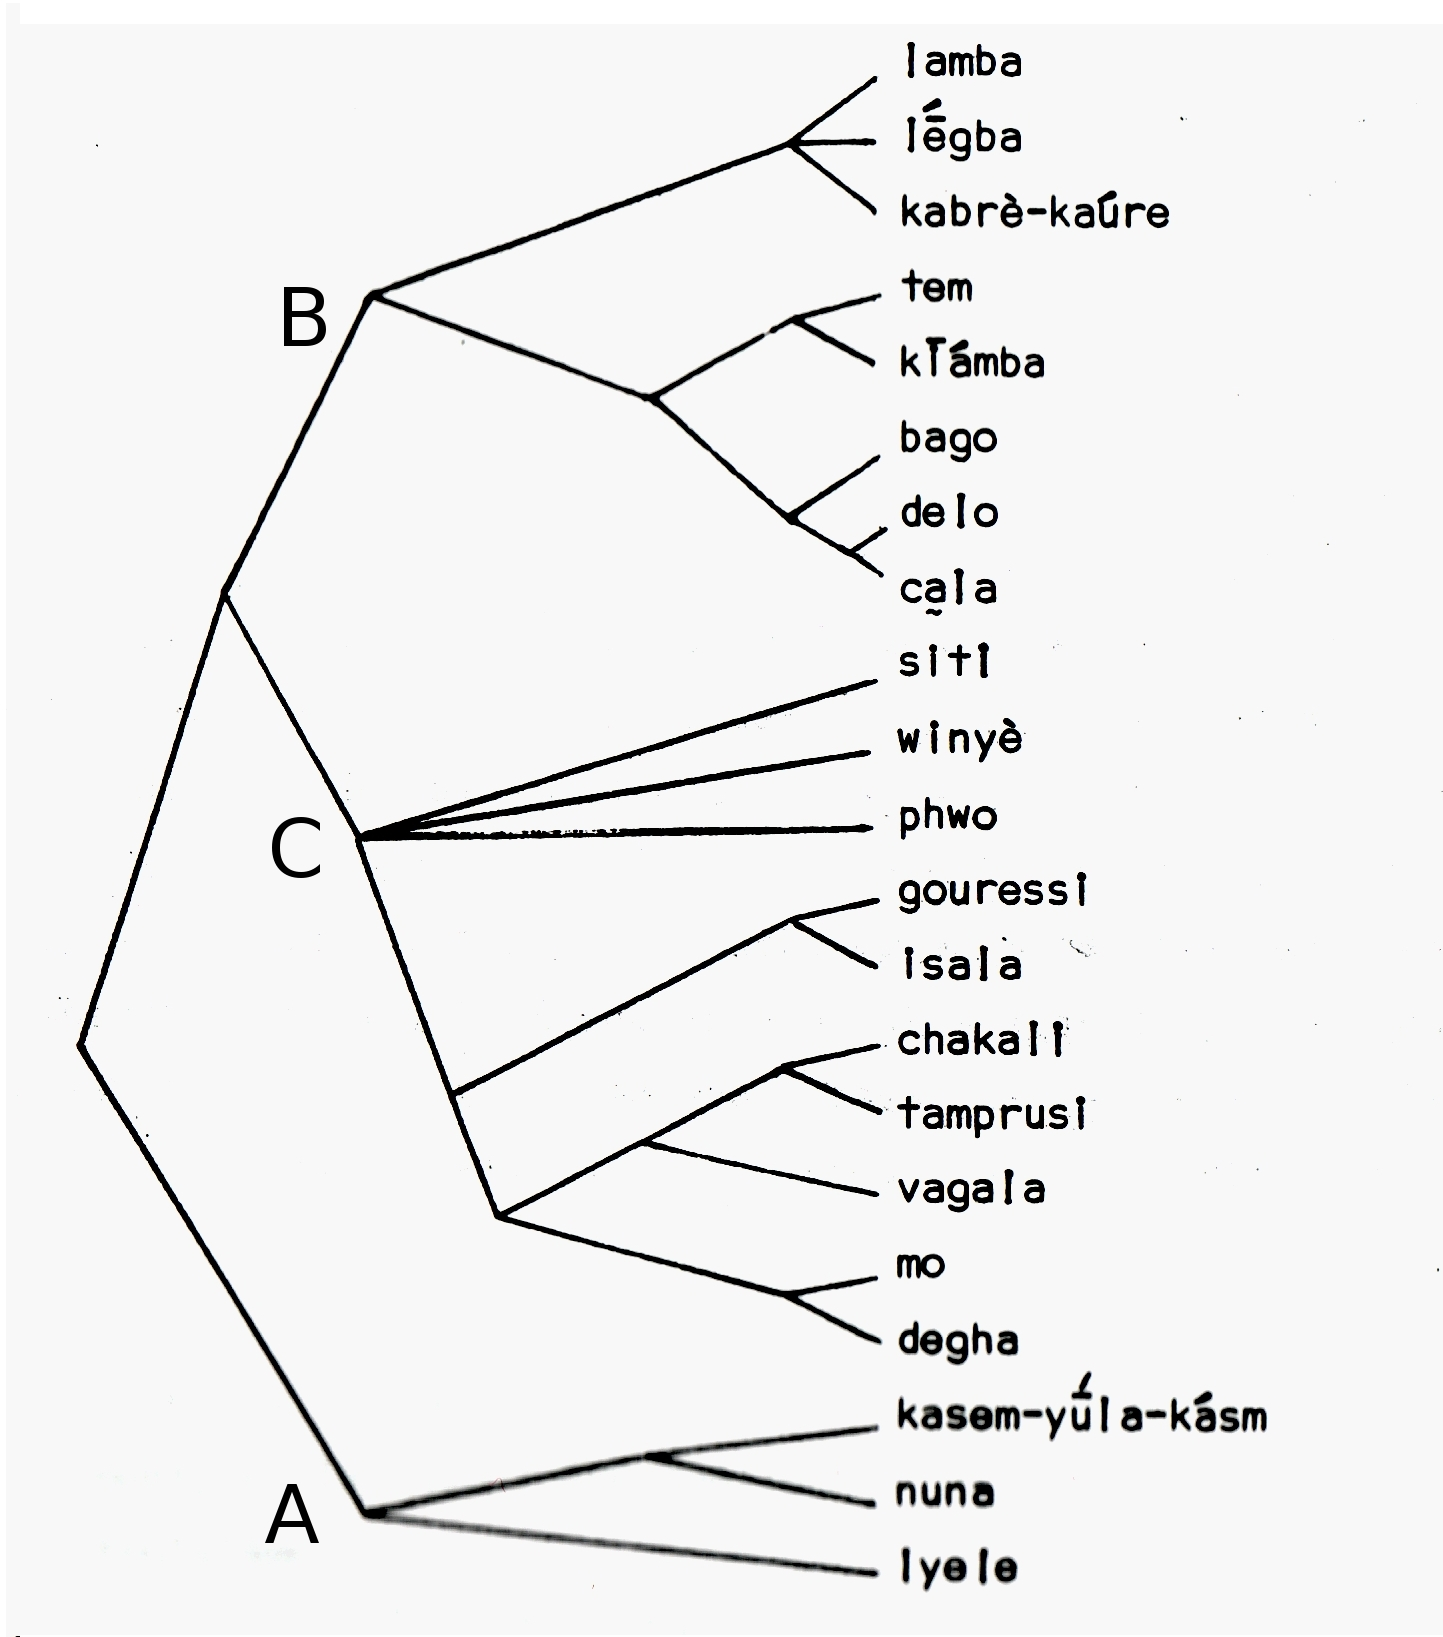
\includegraphics[width=6cm, height=6cm]{Graphic/Pictures/File-0002NEW.jpg}
\caption[Clustering of 
 Manessy]{Clustering of 
\citet[86]{Mane69b} (Modifications JAB)\label{fig:Mane-clust}}
\end{figure}



 In his group C, \citeauthor{Mane69b} clusters
Chakali and Tampulma ({\it tamprusi}), followed in turn by Vagla  ({\it
vagala}) and Dɛg ({\it mo-degha}). The present result, based only on
cardinal numerals,
 is
somewhat corroborated by his Grusi schematisation reproduced in figure
\ref{fig:Mane-clust}. Nevertheless,  what he treats as two languages (i.e. {\it
mo} and {\it degha}) is treated here as one, and Pasaale is not represented.  



\paragraph{Examination using body part terms}
\label{sec:NUM-bodypart}

As a final note, I apply the phonetic comparison method on data from another
semantic domain.  The data  given in table
\ref{tab:NUM-rec-Swad} is  a twelve-member set
of body part terms  taken from the Swadesh-100. 


\begin{table}[!h]
 \caption{Selected items from recent Swadesh-100  \label{tab:NUM-rec-Swad}}
 \centering
 \begin{Itabular}{llllll}
\Hline
 & Chakali & Tampulma & Deg & Vagla & Pasaale \\[1ex] \hline 

skin & tɔ́ŋ & tɔn & tɔ̀ń & hɔŋ & tèŋ \\ 
bone & hóg & hok & hóg & hog & hógó \\
hair &  pʊ́ŋ & pɪn & pʊ́n & hʊŋ & púŋ \\ 
head & ɲúù & nʊha & ɲú & ɲũ & ɲú \\ 
ear & dɪ̀gɪ̀nà & dʊŋna & dɪ́ŋnɪ́ & dɪgnɪ & dɪ́gɪ́ŋ \\ 
nose & mɪ̀ɪ̀sá & miisa & mɪ̀ɪ́ & miizi & mììsé \\ 
mouth & nʊ̃̀ã́ & nɔ & ɲʊ̀á & nua & ɲʊ̃̀á \\ 
tooth & ɲɪ́ŋ & ɲɪn & ɲɪ́n & ɲɪ́ŋ & ɲɪ́ŋ \\ 
arm & nèŋ & nin & nɔ́n & noni & nʊ́ŋ \\ 

breast & ʔɪ́l & ʔɪl & ʔɪ́l & ʔɪla & jɪ́lá \\ 
 neck & bàɣənà & baŋna & báŋá & baŋa & gágɪ́ná \\ 
\Hline
\end{Itabular}

\end{table}




\begin{table}[!h]
\centering
\caption[Distance of selected  Swadesh-100 items]{Calculating the
distance of selected Swadesh-100 items. C: Chakali, T:
Tampulma,
D: Dɛg V: Vagla and   P: Pasaale
\label{tab:NUM-we-sample}}

\begin{Itabular}{lllllllllll}
\Hline
 & CT & CD & CV & CP & TD & TV & TP & DV & DP & VP \\[1ex]  \hline
skin &1&1&1&0.5&0&2&1.5&2&1.5&1.5\\
bone &1&0&0&1&1&1&2&0&1&1\\
hair & 1.5 & 1 & 1 & 0.5 & 0.5 & 2.5 & 1.5 & 2 & 1.5 & 1.5 \\ 
head & 4 & 0.5 & 1.5 & 0.5 & 3.5 & 3.5 & 3.5 & 2 & 0 & 1 \\ 
ear & 1.5 & 1.5 & 0.5 & 3 & 1 & 2 & 4.5 & 1 & 4 & 3 \\ 
nose &1&2&2.5&1.5&3&1&0.5&3&3&1.5\\
mouth & 1.5 & 1 & 0 & 1 & 2.5 & 1.5 & 2.5 & 1 & 0 & 1 \\ 
tooth &1&1&0&0&0&1&1&1&1&0\\
arm &1.5&1.5&2.5&0.5&0.5&1.5&1.5&1.5&1.5&2.5\\
breast & 0 & 0 & 1 & 2 & 0 & 1 & 2 & 1 & 2 & 1 \\ 
neck & 2 & 3 & 3 & 1.5 & 2 & 2.5 & 3 & 0 & 4 & 4  \\[2ex]  \hline


SUM &16&12.5&13&12&14&19.5&23.5&14.5&19.5&18 \\ 
\Hline
\end{Itabular}
\end{table}



In table \ref{tab:NUM-we-sample},  the pair  Chakali-Pasaale shows the least
distance to one another,  i.e.  the lowest values 12, followed  by
the pair Chakali-Dɛg   (value 12.5). Notice  the close
distance between these and the clusters Chakali-Vagla (13) and  Tampulma-Dɛg
(14).  This result reveals that (i)  the clusters SSWG and NSWG almost vanish
when body part terms are used
as the semantic domain,  (ii) among all pairs Chakali enters into, the
pair Chakali-Tampulma has the highest value, and (iii)
the pair  Vagla-Dɛg is not among the  ones with the lowest value (i.e. value
of 14.5). 

\subsection{Discussion}
\label{sec:NUM-clust-eval}


To summarize, I take advantage of less correspondence items than
\citeauthor{Bend65} and \citeauthor{Mane69b} to cluster the five languages, i.e.
97 and 36 items respectively compare to 10 for numerals and 11 for body part
terms. The limited number of words compared
may be seen as a drawback in my approach, but I believe that a favorable
position is to make use of each word as multi-data points and to compare the
words of a single conceptual domain.  An  advantage is that
 the procedure used here to calculate the distance is stated and allows for
future refinements, unlike the lexicostatistics used by
\citeauthor{Bend65}.\footnote{The question I have in mind is where does  one
draw the line between ``look-alike''  and  ``not-look-alike'' words.} 


Another advantage of this
approach is that when the  results of comparing  semantic domains
differ, it can support claims such as  one language has been more
conservative,  has undergone different external influences, or
shows a particular trend in
cultural development than others. This is in fact what happens when numerals and
body part terms were compared. Accordingly, I have shown that: (i) for a
dataset consisting of
items referring to the cardinal numerals, the closest language to Chakali is
Tampulma, and (ii) for a dataset consisting of body part terms,
the closest languages to Chakali are Dɛg and Pasaale. 


\paragraph{On higher numerals}
\label{sec:NUM-high-num}


It is common to read that borrowing into numeral system is more likely to occur
for higher numerals than for lower ones. As \citeauthor{Ratt32a}, and many
others, has written: 

\begin{Quote}
Words used for numerals appear among the least constant and the most subject to
borrowings, more especially among the higher numbers.
\end{Quote} \Source{\cite[114]{Ratt32a}}
 
Possible reasons are proposed in
\cite{vonM10}. I believe that borrowing is the source of the present forms for
100 and 1000 in the five languages.  In fact, the expressions conveying the
numerals 20, 100 and 1000 in all Western
Grusi languages do not seem to be typical Grusi, but resemble  the
corresponding expressions of other  languages, usually
languages with whom the speakers are/were under chieftancy, sharing land or
 involve in socio-economic
relations.   It appears more likely that the genesis of most of SWG higher
numeral involves diffusion from non-Grusi sources, rather than from  common SWG
descents. I believe that higher numerals in this linguistic area have two
origins: one is Oti-Volta and the other is Gonja. 
%For instance, Winyé's higher numerals are similar to those in Manding
%languages
The  forms for 100 and 1000  in Vagla and Dɛg  are similar
to Gonja's forms with the same
denotation, i.e. Gonja {\S  kɪ̀làfá} 100 and  {\S  kíɡ͡bɪ́ŋ} 1000.  Similar
form-denotation can be found in other North Guang languages (e.g.
Krache, Kplang, Nawuri, Dwang and Chumburung) and {\S lafa} is found in many
other Kwa languages, as well as  non-Kwa languages, e.g. Kabiye (Eastern
Grusi)  \citep{Chan09}. Borrowing is  supported by the claim that the Vaglas
and Dɛgas were where they are today before the arrival of the Gonjas
 (\citet[12-13]{Good54}; \citet[516]{Ratt32a}), and the fact that they, but
mostly the Vaglas, are still in contact with the former conquerer, the Gonjas. 

Of all Western  Oti-Volta languages, the Tampulmas have had more contact with
Mampruli  than any other, whereas the Chakali and the Pasaale
with Waali, a language close to  Dagbani and Dagaare, all of them classified as
Western  Oti-Volta languages. Variations of Manessy's {\it oti-volta commun}
reconstructed forms {\S *KO / *KOB}  `hundred'  and {\S
*TUS}  `thousand'  are found
distributed all over Northern
Ghana, cutting across genetic relationship.  It seems that the two high
numerals are areal features spread by Western  Oti-Volta languages,   and that
Chakali, Pasaale and Tampulma speakers may  have borrowed them from languages 
with which they had the most contact, i.e.   Waali, Dagbani, Dagaare and 
Mampruli.



%%%%%%%%%%%


\paragraph{On opacity}
\label{sec:NUM-opacity}



Along the way I have deliberately ignored number 8  and 20. The
 reason
is that for some of the numerals their internal compositions are hard
to analyse;  they display too much variation or  no sensible interpretation
can be confirmed.  

\citet[166]{Nade89} states that the word
corresponding to `eight' in Vagla  should be analyzed as `2 times 4'.   There is
no doubt that the two last syllables of the Tampulma  and Vagla
words for `eight'  are  similar to their respective forms for the
number `four'. Yet four points lead us to treat them as atom,  as opposed to
the 
complex `2 times 4' proposed by Naden. First,  if `four' is involved, why does
the vowel of the last syllable change in
both languages, i.e. Vagla  {\S naazʊ}  4,  {\S ŋmantannaazi}  8,  and 
Tampulma {\S
naasi}  4, {\S ŋmɛnaasa}  8?  Since the
same phonological domain is involved in both cases, {\sc atr}- or {\sc
ro}-harmony is not an
option to explain the change of vowel quality. That is because in both languages
the vowel quality
in the plural suffixes is usually determined by the nominal root, which is the
same in
both
cases.   Second, it is  usually the base which gets multiplied, so we expect 4
in  `2
times 4'   to be the multiplicand, i.e. [4 $\cdot$ 2]. That is, assuming that 4
is a non-serialized
base, why is the general SWG order {\sc multiplicand} $\cdot$ {\sc
multiplier} violated? Or
did Vagla retain a former base-2 system?  That is improbable.  In addition, 
 the data in table \ref{tab:NUM-SWG-card-num-data} shows that for
multiplication the
value of the left
daughter is always higher than the one of the right daughter. Therefore,  [2
$\cdot$ 4]  goes
against that generalization. Thirdly, if instead  4 was only doubled, you 
would expect a formal exposition, e.g.  reduplication, or a predicate meaning
`double' of some sort. I was not able to find a form {\S ŋmanta}  or  {\S
ŋmɛn} with such a meaning. Fourthly, it could be that the source is not `four',
but `limb' or `leg'. Both
languages have {\S naa} for `limb' or `leg', i.e. Vagla {\S naa} {\it sg.}, 
Tampulma 
{\S naa} {\it sg.}.  One of the plural markers in Tampulma and  Vagla is  {\S
-sV}
and   {\S -zV} respectively.  The form {\S naazi} is the plural  of {\S naa}
`leg (including foot)' in Vagla.  Thus a
potential mutation for Vagla may be  {\S a nandar naazi} `the spider's legs' >
{\S ŋmantannaazi} `eight'. Recall that  Chakali {\S ŋmɛŋtɛl} is
heterosemous/homonymous with the word for `spider' (i.e. an insect with eight
legs).  The last scenario is far-fetched but worth 
closer inspection. This led me to treat  the number  `eight' in
Vagla as an atom, and I decided  not to align the five languages  for
comparison due to their opacity.\footnote{However the `2 times 4' analysis gains
in pertinence when
 evidence from  Eastern Grusi is considered.  Among the twenty-three Grusi
languages,  three of the Eastern Grusi seem to have traces of `four' in their
word for `eight' according to the researchers providing the data in
\cite{Chan09}.  Chala {\F -la}; 2,   {\F -náárá}; 4,   {\F
jiŋináárá}; 8  as ( 4 + 4 ). ``The number 8 might be derived from 'double
four'.'' (donor: Dr.  Ulrich Kleinewillinghöfer).  Lamba  {\F násə̂l}; 2, {\F
násə́násá}; 4,  {\F násə́nnásá}; 8 ( 4 + 4 ?).  Delo  {\F ala}; 2, {\F
anaara}; 4,  {\F ɡyanaara}; 8 ( 2 x 4 ?).}



In terms of alignment,  SWG languages show no resemblance in terms of 
their expressions for the number 20. In Tampulma  and Dɛg, I suggest that
the forms for 20 originate from complex expressions of the type  `twice ten',
i.e. 10$\cdot$2.   Tampulma {\S fumlɛ} and Dɛg {\S fifraanɛ}  both contain a
sequence resembling their
respective forms for the number 2  (i.e. Tampulma {\S fum-lɛ} 20, {\S  lɛɛwa} 2
and Dɛg
{\S fifraa-nɛ} 20, {\S
nɛ} 2).  Logically, a form with the value 10 is expected but
both
languages have the form {\S fi} for 10 and not {\S fum} or {\S fifraa}.
Nonetheless the
latter two forms are treated as a consequence of plurality, that is, in Tampulma
and Dɛg, 20 is not an atomic expression but (originates from) a complex one of
the type 
10$\cdot$2.  I  treat  Tampulma's  {\S fum-} as the plural form of {\S fi},
but it is more likely to be  a frozen form than a morphological
operation. The language Kasem is similar to Tampulma; the serie [21-99] is
decimal, the
form for 10 is {\S fúgə́}  and for 20 {\S  fííǹlè}, i.e. 10$\cdot$2 is
expressed {\S fúgə́}$\cdot${\S le} \citep[158]{Bonv88}. The Dɛg sequence
{\S
fifraanɛ} is analysed as  `twice the repetition of ten', i.e. {\S fifraanɛ} <
{\S fi$\sim$fi anɛ}.   The expression for 20 in Vagla was probably borrowed from
Gonja and is treated as an atom.\footnote{Gonja probably borrowed it from Akan.
A {\F taku}  was an Akan weight of slightly higher value than the {\F damma},  a
tiny unit of gold dust \citep[117.fn16]{Wins07}. Around  the same period {\F
taku} referred also to a string of cowries. In 1784, a {\F taku} was worth 20
cowries (Winsnes {\it ibid}), but the amount was subject to the economy of a
specific time, and changes from text to text.   This word may have a Coast
Portuguese origin according to \citet[333]{John70b}.  The expression {\F
kòtòkùó nùm} in Akan, {\it lit:} five sacks, used to refer to a thousand
old cedis. This is identical in meaning and composition to Chakali. However, to
hear this expression today from Akanophones might be difficult,
but similar expressions are frequent and constitute an essential aspect of  base
expressions in numeral systems used for currency in many places of Northern
Ghana.} Caution should be taken since {\S
toko} was and is present in many languages of Ghana, especially in the domain of
currency, and
does not necessarily mean `twenty'. Chakali and Pasaale share a
similar first
CV syllable, i.e.  {\S ma} and  {\S mɔ} respectively. This syllable seems to
come from the Sisaala neighborhood. This is suggested by the data in table
\ref{tab:Sisaala-high-numerals}. 



\begin{table}
\centering
\caption{10, 20, 100 and 1000 in the dialects of Sisaala (source \cite{Chan09})
\label{tab:Sisaala-high-numerals}}
 \begin{Itabular}{l|llll}
\Hline
& Pasaale [sig] & Tumulung  [sil]& Western  [ssl] & Sisaala  [sld]\\ \hline

10& fí&fíí&fíí&fí\\ 
20& mɔ̄líjà & màrá& mɛ̀rɛ́& mɛ́rɛ́\\
100 &kɔɔ&zɔ̀lɔ́ & zɔ̀lɔ́ & zɔ́lɔ́\\
1000&tʊ́sì& bʊ̀ɪ́& bʊ̀ɪ́ & bʊ́ɪ́ \\
\Hline
 \end{Itabular} 

\end{table} 



The last syllable of the
expression for 20 in Pasaale resembles its  form for 2, i.e. {\S lija}.
Nevertheless,
I  prefer to treat Pasaale {\S mɔlija} and Chakali {\S matʃeo} as atomic. In
Chakali and all the dialects of Sisaala, the verb `to attach' or   `to stick
together' is expressed with  a variant of {\S mara}.\footnote{One could imagine
an etymology in which `attach' is central. In a
number of  oral reports, I heard that both cowries and
some British
West African coins (i.e. the tenth of a penny, the one-half penny and the one
penny, that is those with holes in them) were put on strings for conveyance.} 






\subsection{Summary}
\label{sec:NUM-compar-discuss}



 By limiting ourself to  five SWG languages and  comparing  words of  a
defined conceptual domain, the approach presented here
diverges from mass
comparison (i.e. many languages, few words from mixed domains) and
the traditional
method (i.e. few languages,  many words from mixed domains). As a method of
synchronic comparison I suggest a refinement on ordinary
lexicostaticstics as far as the comparison of look-alikes is concerned. More
importantly I do not claim this  has diachronic significance, even though it
would be possible to extrapolate  based on the various clusters.  What it does
is provide a useful measure of how synchronically different the number systems
are
today. 

In spite of that, there are several problems I would like to mention in
conclusion.   First, the cost
calculation of phonetic comparison suffers from its generality and ignores
basic features and domains. The method ignores 
whether a sequence of vowels is due to internal
development from a single vowel or loss of a medial consonant.  Also,  a
medial consonant
should definitely carry less weight than an initial consonant since  many
consonants in medial position are known to systematically change. It should be
possible to weight the consonants and vowels according to whether it is known
that
a difference is due to a regular sound change since the most recent common
ancestor of SWG.  Overall, the method must be designed with 
more representive  costs than those presented in section \ref{sec:NUM-method}. 


Second, to say that a set of forms and their proper combination constitute a
numeral system {\it of a language} is to assume that a language is an abstract
ideal. This is the position taken here: my Chakali data are from Ducie
and I know that in Ducie {\S sandoso} and {\S dɪɡɪtʊʊ} are both used to
express the number 9,  the former by a minority.  Yet this position ignores
important subtilities which  affect the  description, and thus an
explanation. By comparing the five languages,   
finer distinctions existing within those languages are not reflected. There
are 
(folk-linguistically) well-known dialectal variations between the Tampulma East
and West of
the Konkor escarpment, Northern and Southern dialect of Dɛg,  Pasaale of Kundugu
and
Jaala and Pasaale of Funsi, Jumo and Bufiama, the Chakali tri-partition
discussed in chapter \ref{sec:SOC-lingvit}, among possibly  others.
My  point is that selecting a form to
represent a language affects the overall results in a non-controllable way. 
Unless a researcher knows
the origin of the data (i.e. where, when and who), the results 
indicate
rather than conclude. 





Whereas the normalization of the consonants are unequivocal, the vowels are
analysed as they are presented. Nonetheless there are cases which seem dubious.
The phonological system of each language, apart from Chakali, has been
studied and appears in a series of phonological
descriptions published under the title   \textit{Collected Language Notes} (i.e.
\cite{Crou66, Gray69, Toup95,  Crou03}). As discussed in section
\ref{sec:LOW-phon-vowel}, the vowel inventories are always either of nine
or of ten phonemes  in
these
descriptions,  only contrasting for the low vowels.  All five
SWG languages  have four {\sc +hi} vowels, discriminated by the features {\sc
 ro} and {\sc
atr}. It is likely  that
some of the data donors in \cite{Chan09} do not render the distinctions in
their transcription.
Two factors could be
responsible for the absence of such a distinction, for instance transcribing 
{\S ʊ} $>$  {\S o},
{\S ʊ} $>$ {\S u},  {\S ɪ} $>$ {\S e} or {\S ɪ} $>$ {\S i}: (i) the contrast is
not perceived by the researcher and
thus
the contrast is not reflected in the data, or (ii) the transcription is based on
a conventionalized alphabet designed for literacy. I believe the latter factor
is the one responsible for the present state of the data, especially in the case
of Tampulma. Another way to identify a less reliable transcription  is to
discover an {\sc atr} disagreement.  As discussed in section
\ref{sec:vowel-harmony},  among the SWG languages, and, to a
certain
extent, across the Gur group, {\sc atr}-harmony is a recurrent typological
characteristic, i.e. vowels in a certain domain must share the same value for
the
 harmonic feature {\sc atr} \citep{Casa03}. This method is not infallible as
there are often no way
to prove from the data at hand that the domain in a given word is in fact
operational for  {\sc atr}-harmony.  Therefore, the clustering of SWG languages
(and
its
reconstruction)  should not rely first on evidence provided by vowel
qualities.\footnote{See
\citet[509-510]{Casa08} for thoughts on the auditory confusion of field
linguists who are not themselves native speakers.}

Related to the previous point, it is important to keep in mind that a 
transcription is an analysis, and,  given the state of documentation of the SWG
languages, often the only one available. There is an unresolved problem
in SWG which has been identified as the ``suspect sequence''  in    the 
\textit{Collected Language Notes} cited above. It consists of the representation
of the sequences of vowels in which the first is a {\sc +hi, -ro} vowel.
What is important here is that  the number 2 in Pasaale is transcribed {\S
bàlìyà},
and the Chakali cognate  is transcribed  {\S álìɛ̀}. Are the sequences {\S
iya} and {\S ɪɛ} `really' different or are they the result of  a transcription
convention?  Depending on this detail alone, the method of phonetic comparison
can treat 
Chakali
and Pasaale  either at a distance of 1 or 3  (see figure
\ref{fig:NUM-align-quant-two-EXE}).  Such a difference
in value resulting from a non-representative transcription
convention  obviously affects the overall result in an artificial way. 


















\begin{landscape}
\begin{center}
\footnotesize{
 
\tablefirsthead{%
\Hline
 & Chakali  & Tampulma  & Dɛg & Vagla  & 
Pasaale\\[1ex] 
\hline}

\tablehead{%
\hline
\multicolumn{6}{l}{\textit{continued from previous page}}\\
\hline
& Chakali  & Tampulma  & Dɛg & Vagla  & 
Pasaale\\[1ex] \hline
}
\tabletail{
\hline
\multicolumn{6}{r}{\textit{continued on next page}}\\
\hline}
\tablelasttail{\hline}
\topcaption{SWG cardinal numeral data \citep{Chan09}
\label{tab:NUM-SWG-card-num-data}}

 \begin{xtabular}{llllll}

1 & dɪ́ɡɪ́máŋá & diiɡɛ & beŋk͡paŋ   & k͡páŋ  & kɪ́dɪ́ɡɪ́   \\ 
2 & álɪ̀ɛ̀ & alɛɛwa &  anɛ   & ànɛ̀ɛ̀ & bàlìyà  \\ 
3 & átòrò  & atoora &  atoro  & àhòrò  & bòtò  \\ 
4 & ànáásɛ̀ & anaasi  &  anaarɛ   & ànáázʊ̀  & bànāā  \\ 
5 & āɲɔ̃̄ & anyuún &  anue  & ànúè  & bɔ̀nɔ̀ŋ  \\ 
6 & álòrò & anɔɔrà &  anʊmɛl        & ànʊ́mbɛl  & bàdʊ̀  \\ 
7 & àlʊpɛ̀  & anɔpɛ &  anʊanɛ      & àníídàànɛ̀ɛ̀  & bàpɛ̀  \\ 
8 & ŋmɛ́ŋtɛ́l & ŋmɛnaasa  & anʊatoro  & ámàntánnààzí / ŋmàntánnààzí  
& kyórí  \\ 
9 & dɪ́ɡɪ́tūū / sandoso & diɡtó  & anʊanaarɛ  & kábɛl  & níbí  \\ 
10 & fí & fí & fi & fí & fí  \\ 
11 & fí di dɪ́ɡɪ́(máŋá) & fidikibɛɡím & fi dɛ beŋk͡paŋ  & fídɪ̀k͡páŋ  &
fí béé kɪ́dɪ́ɡɪ́   \\ 
12 & fí di álìɛ̀ & fiidaalɛ́ & fi dɛ anɛ & fídàànɛ̀ɛ & fí béé bàlìyà
\\ 
13 & fí di átòrò & fiidaatora & fi dɛ atoro & fídààhòrò & fí béé
bòtò  \\ 
14 & fí di ànáásì & fiidaanaasí & fi dɛ anaarɛ & fídàànáázʊ̀ & fí
béé bànāā  \\ 
15 & fí di āɲɔ̃̄ & fiidaanyuún & fi dɛ anue & fídàànúè & fí béé
bɔ̀nɔ̀ŋ  \\ 
16 & fí di álòrò & fiidaanɔ́ra & fi dɛ anʊmɛl & fídàànʊ́mbɛl /
fídàànʊ́mal & fí béé bàdʊ̀  \\ 
17 & fí di àlʊpɛ̀ & fiidaanɔ́pɛ & fi dɛ anʊanɛ & fídààníídàànɛ̀ɛ̀ & fí
béé bàpɛ̀  \\ 
18 & fí di ŋmɛ́ŋtɛ́l & fiwaŋŋmɛnaasà  & fi dɛ anʊatoro &
fídìàmàntánnààzí   & fí béé kyórí  \\ 
19 & fí di dɪ́ɡɪ́tūū & fiwadiɡtó  & fi dɛ anʊanaarɛ  & fídìkábɛl  & fí
béé níbí  \\ 
20 & màtʃéó & fumlɛ & fifraanɛ & tòkkò & mɔ̄líyà \\ 
21 & màtʃéó anɪ dɪ́ɡɪ́máŋá & fumlɛdikibɛɡím & fifraanɛ dɛ beŋk͡paŋ  &
tòkkò ní k͡páŋ & mɔ̄líyà béé kɪ́dɪ́ɡɪ́  \\ 
22 & màtʃéó anɪ álìɛ̀ & fumlɛdaalɛ́ & fifraanɛ dɛ anɛ & tòkkò ní ànɛ̀ɛ̀
& mɔ̄líyà béé bàlìyà  \\ 
23 & màtʃéó anɪ átòrò  & fumlɛdaatora & fifraanɛ dɛ atoro & tòkkò ní
àhòrò & mɔ̄líyà béé bòtò  \\ 
24 & màtʃéó anɪ ànáásì & fumlɛdaanaasí & fifraanɛ dɛ anaarɛ  & tòkkò
ní ànáázʊ̀  & mɔ̄líyà béé bànāā  \\ 
25 & màtʃéó anɪ āɲɔ̃̄ & fumlɛdaanyuún & fifraanɛ dɛ anue & tòkkò ní
ànúè & mɔ̄líyà béé bɔ̀nɔ̀ŋ  \\ 
26 & màtʃéó anɪ álòrò & fumlɛdaanɔrà & fifraanɛ dɛ anʊmɛl & tòkkò ní
ànʊ́mbɛl & mɔ̄líyà béé bàdʊ̀  \\ 
27 & màtʃéó anɪ àlʊpɛ̀ & fumlɛdaanɔ́pɛ & fifraanɛ dɛ anʊanɛ & tòkkò ní
àníídàànɛ̀ɛ̀ & mɔ̄líyà béé bàpɛ̀  \\ 
28 & màtʃéó anɪ ŋmɛ́ŋtɛ́l & fumlɛŋmɛnaasà  & fifraanɛ dɛ anʊatoro & tòkkò
ní ŋmàntánnààzí   & mɔ̄líyà béé kyórí  \\ 
29 & màtʃéó anɪ  & fumlɛdiɡtó  & fifraanɛ dɛ anʊanaarɛ  & tòkkò ní kábɛl
 & mɔ̄líyà béé níbí \\ 
30 & màtʃéó anɪ fí  & fumtora & fifraatoro & tòkkò ní k͡pɔrɡɔ & mɔ̄líyà
bée fí  \\ 
40 & màtʃéó álìɛ̀ & fumnaasí & fifraanaarɛ & tòkkò ànɛ̀ɛ̀  &
mɔ̀ɭíbàlìyà \\ 
50 & màtʃéó álìɛ anɪ fì & fumnyuún & fifraanue & tòkkò ànɛ̀ɛ̀ nɪ́ fí
/ adunu ( < Gonja )  & mɔ̀ɭíbàlìyà bée fí \\ 
60 & màtʃéó átòrò  & fumnɔrá & fifraanʊmɛl & tòkkò àhòrò  &
mɔ̀ɭɪbòtò   \\ 
70 & màtʃéó átòrò anɪ fì & fumnɔpɛ́ & fifraanʊanɛ & tòkkò àhòrò nɪ́
fí  & mɔ̀ɭɪbòtò bée fí \\ 
80 & màtʃéó ànáásì  & fumŋmɛnnaasá  & fifraanʊatoro & tòkkò ànáázʊ̀
 & mɔ̀ɭɪbànāa  \\ 
90 & màtʃéó ànáásì anɪ fì & fumdiɡtó & fifraanʊanaarɛ  & tòkkò
ànáázʊ̀ nɪ́ fí   & mɔ̀ɭɪbànāa bée fí \\ 
100 & kɔ̀wá & kɔkwa & lafa & kàlfà & kɔ̀ɔ́ \\ 
200 & kɔ̀sá álìɛ̀ & kɔksaalɛ́ & lafranɛ & kàlfà ànɛ̀ɛ̀ & kɔ̀ɔ́ bʊ̀lɪ̀yà 
\\ 
1000 & tʊ̀sʊ̀   & tusuká & kaɡ͡boŋ  & káɡ͡bóŋ  & túsì   \\ 
2000 & tʊ̀sà álìɛ̀ & tusukasaalɛ́ & kaɡ͡boŋ anɛ & káɡ͡bóŋ ànɛ̀ɛ̀ & túsì
bʊ̀lɪ̀yà  \\ 
\Hline


\end{xtabular}
}
\end{center}
\end{landscape}
